% main.tex

\documentclass[a4paper,11pt]{jsreport}
\usepackage{pxrubrica} % ルビ(ふりがな)を使用する場合
\usepackage[dvipdfmx]{graphicx} % 画像の挿入のためのパッケージ
\usepackage{subcaption} % サブキャプションを扱うためのパッケージ
\usepackage{url} % URLの挿入のためのパッケージ
\usepackage{multirow}
\usepackage{comment}
\usepackage{array}
\usepackage{parskip}
\usepackage{otf}
\usepackage{amsmath}
\usepackage{algorithm}
\usepackage{algpseudocode}
\usepackage{fancyhdr}
\usepackage[numbers]{natbib}

\newcommand{\citex}[1]{\citeauthor{#1} (\citeyear{#1})}

\pagestyle{fancy}
\fancyhf{} % ヘッダーとフッターをクリア
\fancyhead[L]{\nouppercase{\rightmark}} % ヘッダー左にセクション名を表示
\fancyfoot[C]{\thepage} % フッター中央にページ番号を表示

\setcounter{secnumdepth}{3} % タイトルにどこまの深さまで番号をつけるか
\setcounter{tocdepth}{3}    % 目次にどこまで表示するか

\DeclareFontShape{JY1}{mc}{m}{it}{<->ssub*mc/m/n}{}
\DeclareFontShape{JY1}{mc}{m}{sl}{<->ssub*mc/m/n}{}
\DeclareFontShape{JY1}{mc}{m}{sc}{<->ssub*mc/m/n}{}
\DeclareFontShape{JY1}{hgt}{m}{it}{<->ssub*hgt/m/n}{}
\DeclareFontShape{JY1}{hgt}{m}{sl}{<->ssub*hgt/m/n}{}
\DeclareFontShape{JY1}{mc}{bx}{it}{<->ssub*gt/m/n}{}
\DeclareFontShape{JY1}{mc}{bx}{sl}{<->ssub*gt/m/n}{}
\DeclareFontShape{JT1}{mc}{m}{it}{<->ssub*mc/m/n}{}
\DeclareFontShape{JT1}{mc}{m}{sl}{<->ssub*mc/m/n}{}
\DeclareFontShape{JT1}{mc}{m}{sc}{<->ssub*mc/m/n}{}
\DeclareFontShape{JT1}{hgt}{m}{it}{<->ssub*hgt/m/n}{}
\DeclareFontShape{JT1}{hgt}{m}{sl}{<->ssub*hgt/m/n}{}
\DeclareFontShape{JT1}{mc}{bx}{it}{<->ssub*gt/m/n}{}
\DeclareFontShape{JT1}{mc}{bx}{sl}{<->ssub*gt/m/n}{}

\begin{document}

\thispagestyle{empty} % ヘッダーやフッターを表示させない

\begin{center}
  \leftline{2023 年度卒業}

    \vspace{2cm}
    
    {\Huge 修士論文}
    
    \vspace{2cm}
    
    {\LARGE 深層学習による動画予測手法を用いたSDO紫外線画像の全球時系列予測}
    
    \vspace{1cm}
    
    {\Large a Time-Series Prediction of SDO Ultraviolet Full-disk Images using a Video Prediction Method with Deep Learning}
    
    \vspace{3cm}
    
    \Large
    \begin{tabular}{|c|c|}
      \hline
      \multirow{3}{*}{所属} & 新潟大学 大学院自然科学研究科\\ &  電気情報工学専攻 情報工学コース \\ & 飯田研究室 \\
      \hline
      氏名 &  佐々木明良\\
      \hline
      学籍番号 & F22C017D\\
      \hline
    \end{tabular}
\end{center}

\clearpage % これにより新しいページに移動


\chapter*{概要}
  太陽活動に起因する激しい宇宙天気の変動は、地球上の電力網や衛星通信などの技術システムに深刻な影響を与える可能性がある。
  そのため、太陽活動の観測と宇宙天気の予測は、人類の社会活動を守る上で重要であり、その予測モデルの開発や、現象のメカニズムの研究は盛んに行われている。
  宇宙天気予報において、NASAのSolar Dynamics Observatory (SDO) をはじめとする観測衛星から得られる観測データが重要な役割を果たしている。
  これらのデータは予測モデルの入力や、専門家による予報の情報源として利用されている。
  
  近年の深層学習の進展により、宇宙天気予報においてもその応用が見られるようになった。
  深層学習モデルは迅速な予測を可能にし、確率論的なアプローチを通じて不確実性を考慮することができる。
  NICTによるDeep Flare Netや、NASAによるDeep Learning Geomagnetic perturbationなど、深層学習を利用した予測モデルは実際に運用されており、宇宙天気予報においてその有用性が確認されている。
  
  宇宙天気による影響から重要な技術システムを保護するには、早期かつ正確な予測が必要である。
  しかし、シミュレーションによる予測モデルや深層学習による予測モデルは、多くの場合、数時間から数日後までの予測に焦点を当てている。
  さらに長い時間範囲での予測が理想であるが、計算資源の制約や、太陽の複雑なシステムに対するモデルの予測能力の限界などの理由により、その実現は困難である。

  そのような背景から、本研究では、深層学習を用いた、未来の太陽画像の生成という新しいアプローチを提案する。
  具体的には、動画予測という技術を用いて、SDO / AIAから得られる全球紫外線画像の予測を試みる。
  本研究により、未知の太陽画像を精度よく再現することができれば、既存の予測モデルの入力データとして利用することができ、より早期の宇宙天気予報の実現に貢献することができると考えられる。

  動画予測とは、動画の一部を入力として、それに続く未来の動画を予測するタスクである。
  CNNを中心とした画像処理技術の進展と、LSTMを中心とした時系列データの処理技術の進展、およびその融合により、近年注目を集めている。
  
  はじめに、Motion-Aware Unitと呼ばれる動画予測モデルを用いて、SDO / AIAの211\AA フィルターから得られた時系列全球データを入力とし、48時間以内の4時間ごとの全球紫外線画像を生成するモデルを構築した。
  生成された予測画像に対し、全球、経度ごと、さらに東側外縁部における輝度強度の再現性を評価した。
  さらに、より詳細な性能評価と比較のために、単純作動回転モデルとの比較を行った。
  全球での平均輝度強度の絶対誤差は、48時間後の予測で3.67\% であり、単純差動回転モデルの絶対誤差である10.2\% よりも低かった。
  経度ごとの評価でも、すべての分割セクターにおいて、48時間後時点での絶対誤差が単純差動回転モデルよりも低かった。
  また、東側外縁部においても、良好な性能を示し、動画予測モデルの高い学習能力が確認された。
  さらに、動画予測モデルが予測に要求する時間は数秒であり、非常に高速に予測画像を生成することができた。

  次に、さらなる性能向上を目的として、211 \AA フィルターの全球画像に加え、171 \AA フィルター、193 \AA フィルターの全球画像を追加し、3波長の入力から211 \AA フィルターの画像を予測するモデルを構築した。
  評価は全実験と同様に行った。
  この実験では、ほとんどの評価指標において、実験1の結果を下回るか、同等の結果となった。
  これは、現在使用してる動画予測モデルのアーキテクチャやモデルの深さでは、3波長の入力に対して十分な学習を行うことができないことが原因と考えられる。

  このような結果から、深層学習を用いた動画予測手法は、未知の太陽全球紫外線像の予測という課題において、有効な手法であることが示された。
  特に、高い時空間的ロバスト性を実現する学習能力や、予測の高速性は、実際の宇宙天気予報において求められる重要な条件である。
  今後、本研究の結果をもとにしたさらなるアプローチや改善手法の検討を行うことで、本研究の成果をさらに発展させることができると考えられる。



\tableofcontents

\chapter{研究背景}

 宇宙天気の地球に対する影響
 宇宙天気の撹乱の原因となる太陽活動
 太陽活動の観測と宇宙天気予報
 宇宙天気予報における紫外線画像の利用と重要性
 紫外線像を利用した宇宙天気予報モデルの先行研究
 研究目的: 数日後の紫外線画像を予測し生成する
 近年の動画予測モデルの登場と発展
 本研究で用いる動画予測モデルの概要

宇宙天気とは、太陽活動に起因する宇宙環境の現象を指し、激しい宇宙天気の変動は地球上の電力網や衛星通信など、人間の技術システムに影響を及ぼすことがある。
太陽の表面や大気における物理現象、特に太陽フレアやコロナ質量放出(CME)などの爆発的なイベントは、地球に到達する高エネルギー粒子や放射線の量を増加させ、宇宙天気の変動に大きな影響を与えることが知られている。
そのため、太陽活動を観測し、宇宙天気を予測することは、人間の技術システムを宇宙天気の影響から守るための重要な課題である。

宇宙天気の予報には、太陽フレアの爆発やCMEの発生を予測するものや、太陽風の地球到達時刻や強度を予測するものなどがある。
これらの予測は、様々な観測機器によって得られる太陽観測データを用いて行われるが、紫外線像はその中でも重要な情報源の一つである。
(DeFN、WindNetの話とか)
\chapter{動画予測}

  \section{動画予測の定義と定式化}

    動画予測は、既知のビデオフレームの系列から未来のフレームを予測するタスクであり、教師なし学習、または自己教師あり学習の一種として位置付けられる。
    このタスクは、時空間的な連続性と一貫性を持つ未来のフレームシーケンスを生成することを目指す。

    \subsection{動画予測モデル}
    動画予測の目的は、与えられた過去のフレームシーケンスから未来のフレームを予測するモデル \( M \) を最適化することである。
    ほとんどの動画予測モデルにおいて、モデルの扱うシークエンスは入力長と出力長の二つに分割される。
    入力長は、モデルが予測を行うために必要な過去のフレームであり、一貫してモデルがその動画の時空間的ダイナミクスを学習するために使用される。
    出力長は、モデルが予測を行う未来のフレームであり、モデルが最終的に生成するフレームシーケンスの一部となり、この部分に対して損失が計算される。
    また、もっとも初めの出力フレーム以降のフレームでは、直前の出力フレームが入力フレームとして扱われる。
    動画予測モデル \( M \) は、出力長として位置付けられるある時間ステップ\( t\) のフレーム\( \hat{X}_{t} \) を生成する際は、その直前までの過去のフレーム \( X_{0:t-1} \) を入力として受け取り、それに基づいてそれに続く未来のフレームを生成する。
    このプロセスは以下のように定式化される:

    \begin{equation}
    \hat{X}_{t} = M(X_{0:t-1})
    \end{equation}

    \subsection{最適化}
    最適化プロセスは、一連の学習データセットを用いて、損失関数Lを最小化するように動画予測モデル\( M \) のパラメータを調整する。
    このプロセスは、以下のように表現される:
    \begin{equation}
    M_{\text{optimized}} = argmin_{M} L(\hat{X}, X)
    \end{equation}
    ここで、\( M_{\text{optimized}} \) は最適化された予測モデルを表す。
    この損失関数は、予測された未来のフレームと実際の未来のフレームとの差異を測定するために使用され、一般的には平均二乗誤差(Mean Squared Error, MSE)が用いられる。これは、予測されたフレームと実際のフレームのピクセル単位の差異を測定する。MSEは次のように定義される:
    \begin{equation}
    MSE = \frac{1}{N} \sum_{i=1}^{N} (X_i - \hat{X}_i)^2
    \end{equation}

  \section{動画予測のための基礎技術}
    動画予測には、複数のフレーム間での時空間的な関連を捉え、未来のフレームを予測する能力が必要である。
    この目的を達成するためには、畳み込みニューラルネットワーク(CNN)、エンコーダ・デコーダ構造、長短期記憶(LSTM)、そしてアテンションメカニズムといった複数の技術が組み合わされる。
    ここではそういった基礎技術群について説明する。

    \subsection{Convolutional Neural Network (CNN)}
      動画予測において、CNNは各フレームの空間的な特徴を抽出する役割を担う。
      動画は時間的な次元を持つ一連の画像であり、各フレームにおける空間的な特徴を理解することは、時間的な次元を解析する前の重要なステップである。

      畳み込みニューラルネットワーク(CNN)は、特に画像認識や動画処理において広く用いられる深層学習の一形態である。
      CNNは、画像の局所的な特徴を捉えるために、畳み込み層とプーリング層を交互に繰り返すことで構成される。
      畳み込み層は画像から特徴を抽出するためのフィルターの役割を果たし、プーリング層は画像の特徴を圧縮する役割を持つ。
      CNNを用いた多くの画像処理アプリケーションにおいては、この畳み込み操作とプーリング操作が連続的に繰り返されることで、入力データの高次元な特徴を抽出することを可能にしている。
      ここでは、その二つの重要な操作について説明する。
    
      \subsubsection{畳み込み}
        CNNの主な特徴は、局所的な特徴を効率的に捉えることができる畳み込み層にある。
        この畳み込み層は、入力された画像から特定の特徴を抽出するフィルターの役割を果たし、これにより画像の特徴を圧縮して表現することができる。
        
        CNNおける畳み込み処理は、入力データに対する特定のカーネルの適用として理解される。カーネルは小規模な行列であり、入力データの局所的な領域に対して適用される。
        この畳み込み操作は、入力データを I、カーネルを K とした場合、以下の式で表される。
        \begin{equation}
          S(i, j) = (I * K)(i, j) = \sum_{m}\sum_{n}I(i+m, j+n)K(m, n)
        \end{equation}
        この操作の様子を図\ref{fig:convolution}に示す。
        \begin{figure}[h]
          \centering
          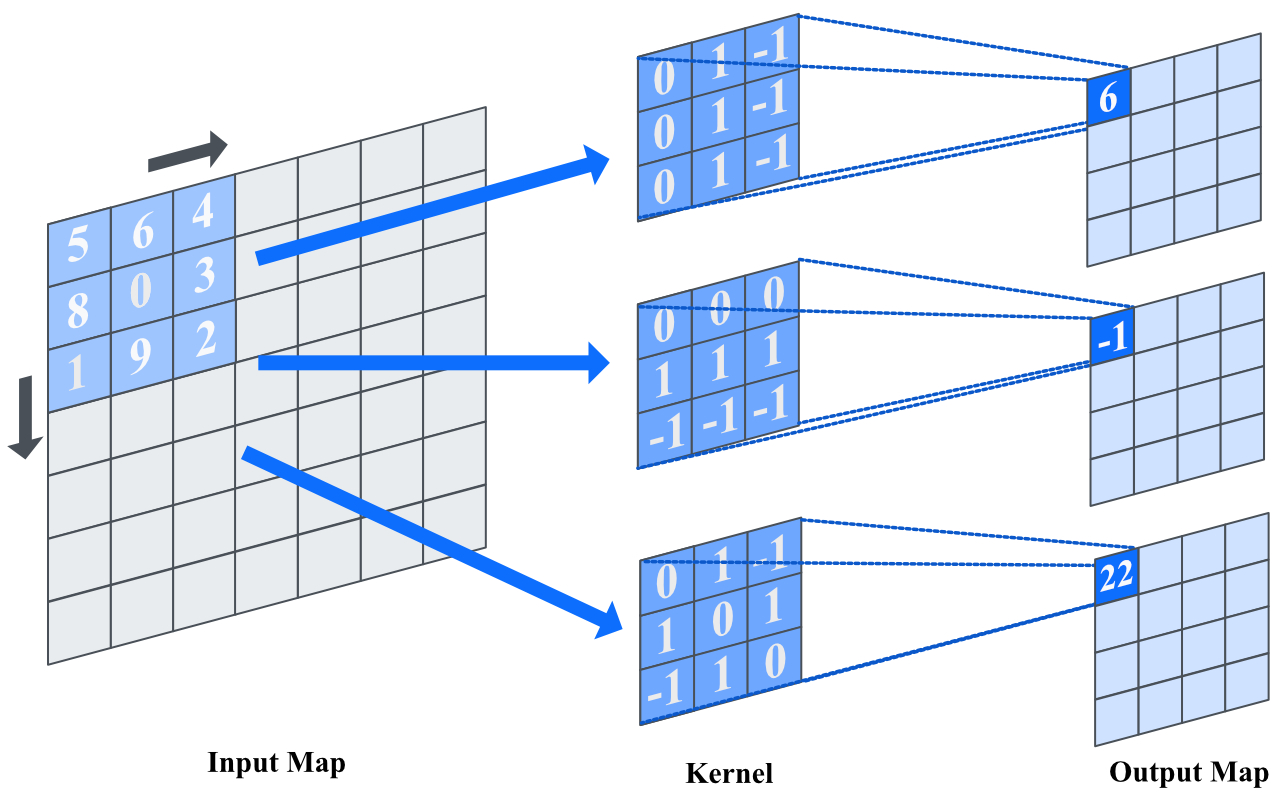
\includegraphics[width=\textwidth]{figures/videoprediction/convolution.jpg}
          \caption{畳み込み操作の様子。左: 入力データ。中央: カーネル。右: 畳み込み操作により生成された特徴マップ。}
          \label{fig:convolution}
        \end{figure}
        この操作は、入力データの全域にわたって繰り返され、最終的に特徴マップと呼ばれる新しい行列が生成される。特徴マップには、その入力データにおける特定のパターンや構造が抽出されている。
      
      \subsubsection{プーリング}
        この層の主な目的は、特徴マップの次元を減少させることである。
        具体的には、プーリング層は特徴マップの小さな領域を集約し、その領域内の代表的な値(最大値や平均値)を抽出する。
        この操作により、ネットワークは画像の局所的な変化に対してより頑健になり、より抽象的な特徴表現を学習することが可能である。

        \begin{itemize}
        \item \textbf{最大値プーリング(Max Pooling)}:この手法では、各領域の最大値が選択される。
        これにより、特徴マップから最も強い信号を保持し、関連性の低い信号を破棄する。
        最大値プーリングは、特に画像内のテクスチャや形状などの顕著な特徴を強調するのに有効である。
        ここで、入力となる特徴マップをF, プーリング領域のサイズをm*n, プーリング層の出力をPとすると、最大値プーリングは以下の式で表される。
        \begin{equation}
          P(i, j) = \max_{m}\max_{n}F(i+m, j+n)
        \end{equation}
        最大値プーリングの様子を図\ref{fig:maxpooling}に示す。
        \begin{figure}[htbp]
          \centering
          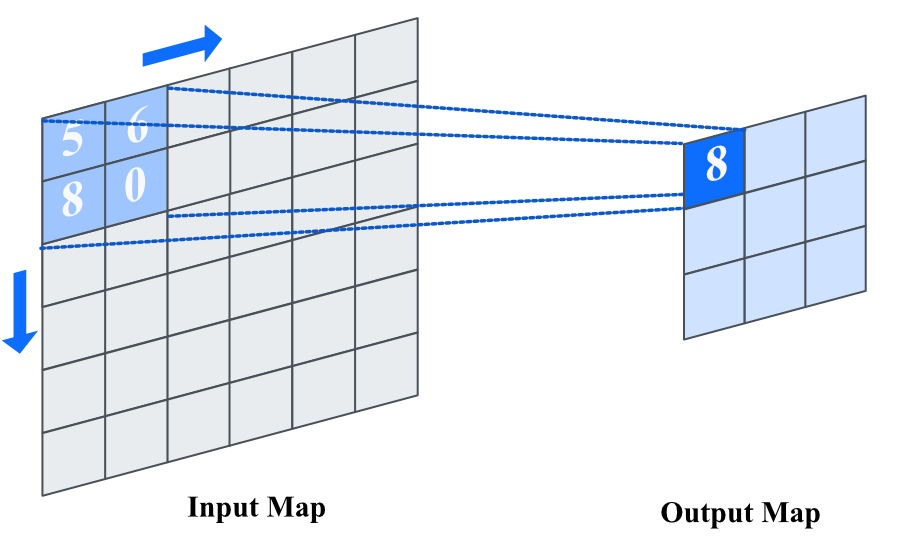
\includegraphics[width=0.7\textwidth]{figures/videoprediction/pooling.jpg}
          \caption{最大値プーリングの様子。左: 入力データ。右: 最大値プーリングにより生成された特徴マップ。}
          \label{fig:maxpooling}
        \end{figure}

        \item \textbf{平均値プーリング(Average Pooling)}:平均プーリングは、各領域の平均値を計算する。
        これにより、特徴マップの全体的な特性をより平滑化し、より均一な特徴表現を提供することが可能である。
        ここで、入力となる特徴マップをF, プーリング層の出力をPとすると、平均値プーリングは以下の式で表される。

        \begin{equation}
          P(i, j) = \frac{1}{mn}\sum_{m}\sum_{n}F(i+m, j+n)
        \end{equation}
        
        \end{itemize}
      

    \subsection{Encoder-Decoder}
      エンコーダ・デコーダ構造は画像処理において広く用いられ、特にU-Netのようなアーキテクチャが代表的である。
      エンコーダ・デコーダ構造は、一連の入力データを処理し、それを内部表現に変換するエンコーダ部分と、この内部表現から出力を生成するデコーダ部分の二つの主要なコンポーネントから構成される。
      動画予測において入力データとなるのは、動画の各フレームであり、出力データはそれに続く未来のフレームである。
      ここでは画像処理におけるエンコーダ・デコーダ構造に焦点を当てて説明する。
        
      \subsubsection{エンコーダ}
        エンコーダは入力データをCNNによって処理し、それを高次元から低次元の表現に変換する。
        このプロセスは、入力データに含まれる重要な情報を抽出し、より扱いやすいサイズまたは形式に圧縮することを目的とする。
        動画予測アプリケーションにおいては、空間的特徴に加え、複雑な時間的特徴の依存性をモデリングするため、一般的な画像処理ディープラーニングモデルと比較して大量の計算資源を必要とする。
        そのため、エンコーダにより特徴を圧縮し、より低い次元で高度な特徴を抽出することは、計算コストの削減という点からも非常に有用である。
        
      \subsubsection{デコーダ}
        デコーダは本質的にエンコーダの逆処理である。動画予測においては、その直前のアーキテクチャにより生成された内部表現を受け取り、目的とする出力を生成する役割を持つ。
        動画予測の再帰ネットワーク内では、エンコーダにより圧縮された行列が扱われるため、そのままでは出力には不適切である。
        デコーダはそのような圧縮された表現を元の次元に展開し、出力に適した形式に変換する。

    
    \subsection{Recurrent Neural Network (RNN)}
    リカレントニューラルネットワーク(RNN)は、時系列データや自然言語などのシーケンシャルな情報を扱うために開発されたニューラルネットワークの一種である\citex{werbos1990backpropagation}。
    RNNの特徴は、過去の情報を隠れ状態として保持し、それを利用して次の出力を生成する点にある。このような再帰的な構造を持つことにより、RNNは時系列性をもつデータを扱うことが可能である。
    RNNの構造を図\ref{fig:rnn}に示す。
    \begin{figure}[htbp]
      \centering
      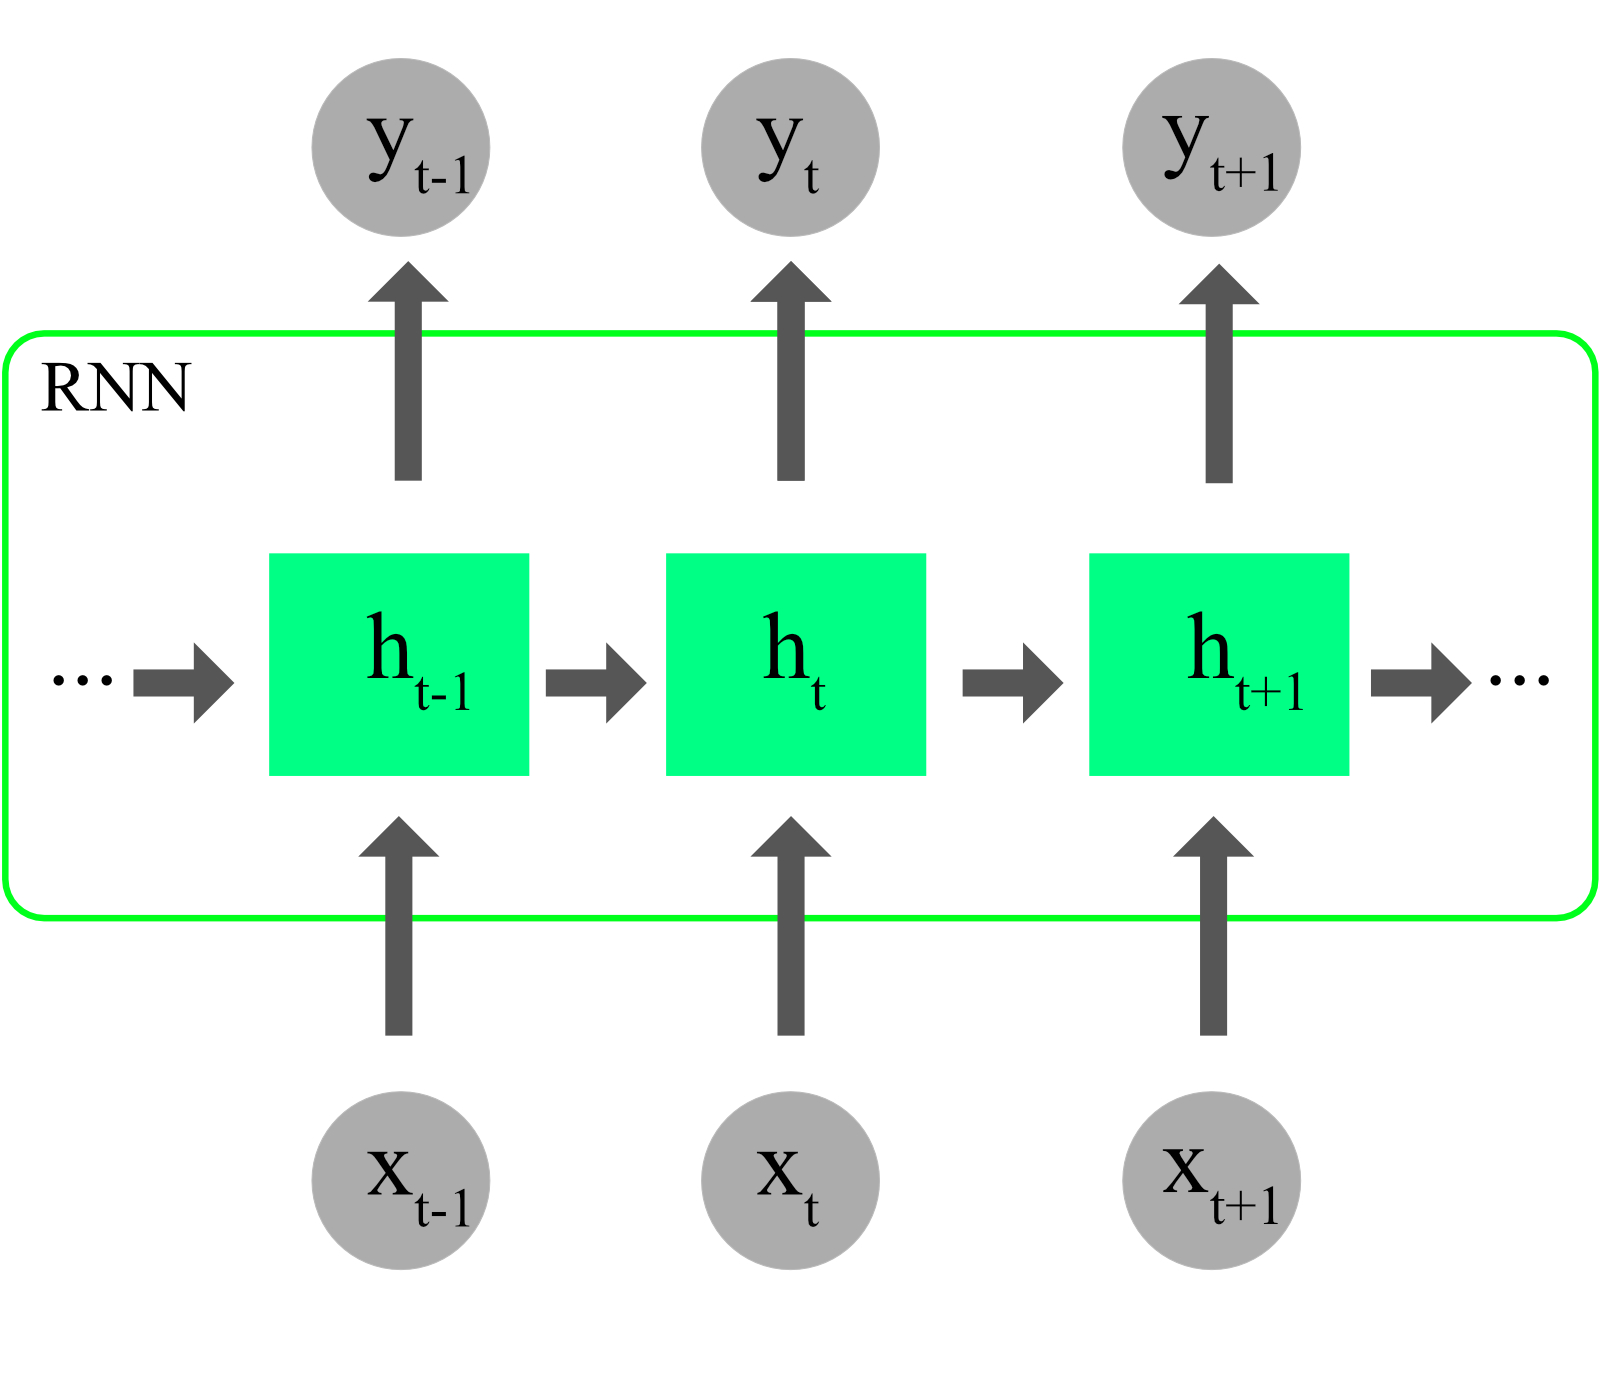
\includegraphics[width=0.75\textwidth]{figures/videoprediction/rnn.jpg}
      \caption{RNNの構造。緑色のブロック\( h \)は隠れ層を表す。}
      \label{fig:rnn}
    \end{figure}
    
    RNNの隠れ層\( h_t \)は、時刻\( t \)での入力\( x_t \)と、\( t-1 \)での隠れ層\( h_{t-1} \)から、以下の式で表される。
    \begin{equation}
      h_t = f(W_{xh} \cdot x_t + W_{hh} \cdot h_{t-1} + b_h)
    \end{equation}
    ここで、\( W_{xh} \)と\( W_{hh} \)はそれぞれ入力と隠れ層の重み、\( b_h \)はバイアスを表し、\( f \)は活性化関数を表す。
    活性化関数には、通常、\( tanh \)や\( ReLU \)などの非線形関数が用いられる。

    このように、RNNは過去の情報を保持することで、時系列データの予測を行うことが可能であるが、実際には、長期的な依存関係を捉えることに困難を抱えていた。
    この問題は「勾配消失問題」として知られる。これは、RNNの活性化関数の出力が各ステップで乗算されることにより、ネットワークが深くなるほど、勾配が指数関数的に消失してしまうことに起因する。
    
    \subsection{Long Short Term Memory (LSTM)}
    この問題を解決するために開発されたのが、長短期記憶(LSTM)である\citex{hochreiter1997long}。
    LSTMは、RNNの基本的な枠組みを保ちつつ、特定の情報を長期間記憶する能力を強化した。
    LSTMの主要な特徴は、セル状態と呼ばれる内部メカニズムであり、これにより長期的な情報を保持することが可能となる。

    LSTMのユニークな構造は以下の三つのゲートから成る:忘却ゲート、入力ゲート、出力ゲート。
    
    1. \textbf{忘却ゲート(Forget Gate)}:このゲートは、セル状態に含まれる情報の一部を削除する役割を担う。
    LSTMネットワークが長期的な依存関係を学習する過程で、関連性の低い古い情報を捨てることが重要である。
    忘却ゲートはシグモイド関数を使用して、どの情報を保持し、どの情報を忘れるかを決定する。
   
    2. \textbf{入力ゲート(Input Gate)}:入力ゲートは、新しい情報をどの程度セル状態に追加するかを決定する。
    このゲートでは、シグモイド関数がどの情報を更新するかを決定し、tanh関数が新しい候補値を生成する。そして、これら二つの値の積が新しい情報としてセル状態に追加される。
    
    3. \textbf{出力ゲート(Output Gate)}:出力ゲートは、現在のセル状態に基づいて、ネットワークの出力を決定する。
    このゲートは、シグモイド関数を使用して、セル状態のどの部分が出力されるべきかを決定し、tanh関数によって処理されたセル状態との積が最終的な出力となる。
    
    LSTMユニットの数学的な定式化は以下の通りである。\( h_t \) は時刻 \( t \) での隠れ状態、\( c_t \) はセル状態、\( x_t \) は入力、\( f_t \)、\( i_t \)、\( o_t \) はそれぞれ忘却ゲート、入力ゲート、出力ゲートの活性化関数を表す。
    \begin{align}
      f_t &= \sigma(W_f \cdot [h_{t-1}, x_t] + b_f) \\
      i_t &= \sigma(W_i \cdot [h_{t-1}, x_t] + b_i) \\
      \tilde{c}_t &= \tanh(W_c \cdot [h_{t-1}, x_t] + b_c) \\
      c_t &= f_t * c_{t-1} + i_t * \tilde{c}_t \\
      o_t &= \sigma(W_o \cdot [h_{t-1}, x_t] + b_o) \\
      h_t &= o_t * \tanh(c_t)
    \end{align}
    
    ここで、\( W \) と \( b \) はそれぞれ重みとバイアスを表し、\( \sigma \) はシグモイド活性化関数、\( \tanh \) は双曲線正接活性化関数を指す。
    LSTMのこの構造により、長期的な依存関係を効果的にモデル化することが可能となり、特に時系列データや動画予測などの分野において有効である。
    LSTMの構造の概念図を図\ref{fig:lstm}に示す。
    \begin{figure}[h]
      \centering
      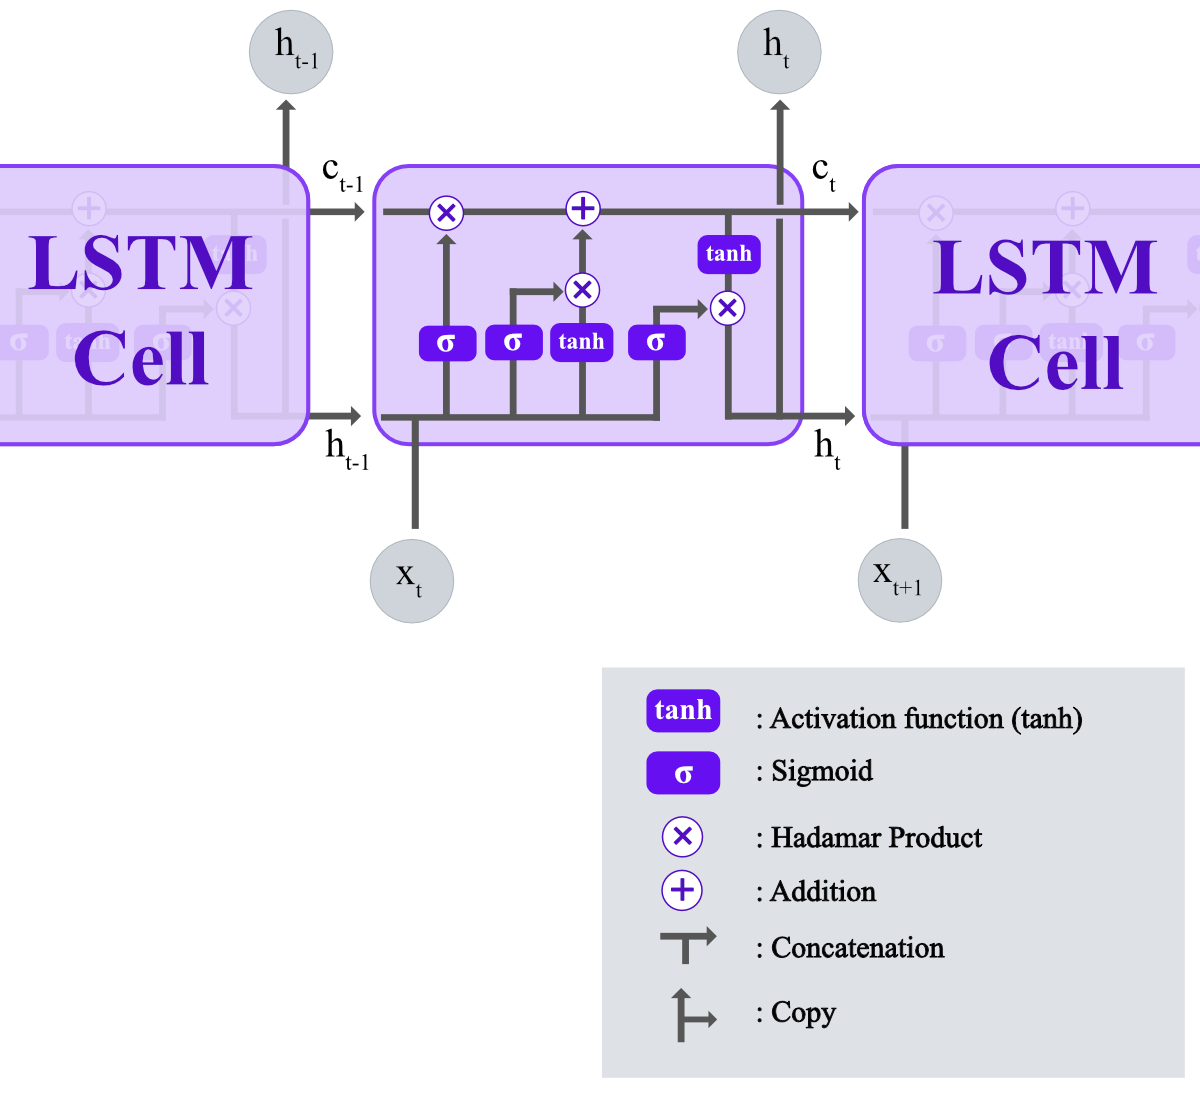
\includegraphics[width=\textwidth]{figures/videoprediction/lstm.jpg}
      \caption{LSTMの構造。}
      \label{fig:lstm}
    \end{figure}
    
    \subsection{Attention}
    アテンションメカニズムは、1990年代に自然言語処理(NLP)分野で初めて提案されたが、
    この技術は、モデルが重要な情報に焦点を当て、それ以外の情報を無視する能力を提供することにより、ディープラーニングにおける重要な進歩の一つとなった。

    アテンションメカニズムの中心には、クエリ(Query)、キー(Key)、バリュー(Value)の三つの概念がある。これらの要素を使用して、モデルがどの情報に注意を払うべきかを決定する。
    \begin{itemize}
      \item \textbf{クエリ(Query)}:クエリは現在注目している要素や状態を表し、モデルがどの情報に注目するかを決定する基準となる。
      \item \textbf{キー(Key)}:キーはデータセット内の各要素に関連付けられ、クエリとの関係を定義する。クエリとキーの間の類似性が高いほど、そのキーに関連付けられた情報に注意が向けられる。
      \item \textbf{バリュー(Value)}:バリューはキーに関連付けられた実際の情報を含み、アテンションメカニズムは、クエリとキーの関係に基づいて、どのバリューを重視するかを決定する。
    \end{itemize}

    アテンションメカニズムの基本的な操作は、クエリと各キーの間の類似性を計算し、それに基づいて各バリューの重み付き和を取ることである。この重み付き和は次のように定義される。
    \begin{equation}
      \text{Attention}(Q, K, V) = \text{softmax}\left(\frac{QK^T}{\sqrt{d_k}}\right)V
    \end{equation}

  \section{動画予測フレームワーク}
    動画予測のフレームワークは、一般的にRNN構造を基本とし、その中にエンコーダ・デコーダ構造やアテンションメカニズムなどの機構を組み込むことで、動画の時空間的な特徴を効果的に捉えることが可能となる。
    ここでは、もっとも基本的な動画予測フレームワークであるConvLSTMと、その後の改良を加えたPredRNN、また本研究で用いるMotion-Aware Unit (MAU) について説明する。

    \subsection{ConvLSTM}
      ConvLSTM(Convolutional Long Short-Term Memory)は、\citex{shi2015convolutional}によって提案された、動画予測とその他の時空間シーケンスデータの処理に特化したニューラルネットワークアーキテクチャである。
      伝統的なLSTMの枠組みを拡張し、畳み込み操作を組み込むことで、空間的な情報を効果的に処理する能力を持つ。
      このような特性により、ConvLSTMは、動画予測のみならず、気象予測や交通流予測など、他の時空間データ処理の応用にも適用可能であり、その応用が期待されている。

      ConvLSTMは、LSTMの各ゲート(忘却ゲート、入力ゲート、出力ゲート)とセル状態の更新に畳み込み演算を導入する。これにより、モデルは時系列データに含まれる空間的パターンを捉え、それを時間的文脈において解析することが可能となる。特に、動画や気象データなどの時空間データにおいて、局所的な空間的特徴と時間的依存関係を同時にモデル化できる。
      ConvLSTMの数学的定式化は以下の通りである。ここで、\( \ast \) は畳み込み演算、\( \circ \) はアダマール積(要素ごとの積)を表す。
      \begin{align}
        f_t &= \sigma(W_{xf} \ast X_t + W_{hf} \ast H_{t-1} + W_{cf} \circ C_{t-1} + b_f) \\
        i_t &= \sigma(W_{xi} \ast X_t + W_{hi} \ast H_{t-1} + W_{ci} \circ C_{t-1} + b_i) \\
        C_t &= f_t \circ C_{t-1} + i_t \circ \tanh(W_{xc} \ast X_t + W_{hc} \ast H_{t-1} + b_c) \\
        o_t &= \sigma(W_{xo} \ast X_t + W_{ho} \ast H_{t-1} + W_{co} \circ C_t + b_o) \\
        H_t &= o_t \circ \tanh(C_t)
      \end{align}

      \( X_t \) は時刻 \( t \) における入力、\( H_t \) は隠れ状態、\( C_t \) はセル状態を示し、\( f_t \)、\( i_t \)、\( o_t \) はそれぞれ忘却ゲート、入力ゲート、出力ゲートの活性化状態を表す。
      \( W \) と \( b \) はネットワークの重みとバイアスパラメータである。この定式化により、ConvLSTMは時空間データの空間的な特徴と時間的な特徴を統合的に処理し、高度な予測を行う能力を持つ。
      ここで、\( N \) はサンプル数、\( Y_i \) は実際のフレーム、\( \hat{Y}_i \) は予測フレームを表す。
      ConvLSTMのユニットの概念図を図\ref{fig:convlstm}に示す。
      \begin{figure}[htbp]
        \centering
        
\includegraphics[width=\textwidth]{figures/sample.png}
        \caption{ConvLSTMの構造。}
        \label{fig:convlstm}
      \end{figure}

    \subsection{PredRNN}
      最初の動画予測モデルであるConvLSTMの発表後、そのアーキテクチャを基に様々な改良が加えられてきた。
      本研究で用いるMotion-Aware Unitの基礎となるPredRNNは、その中でも特に代表的なモデルである。

      \citex{wang2017predrnn}によって提案されたPredRNNは、ConvLSTMを基盤としながらも、いくつかの重要な進化と改良を経て開発された。
      ConvLSTMはセル状態は各層レベルに対して独立であり、時間方向でのみ更新される。このような状況では、最下層は直前の時間ステップの最上層が生成したセル状態を考慮することができない。
      PredRNNではこの概念を拡張し、メモリ状態を異なる層の間で効果的に伝達することを可能にする。
        
      \subsubsection{時空間メモリフロー}
        PredRNNでは、時空間メモリフローを利用して空間情報の伝達を最適化する。このメモリフローは、遠隔状態間で情報を伝達し、勾配消失問題を軽減するために設計されている。
        時間方向と、各時間ステップでの隠れ層方向にジグザグにメモリを流す。
        このように、層をまたいで情報を上方向に伝達し、時間を超えて前方向に情報を伝達することにより、空間情報の効率的な流れを実現し、動画フレーム間のより詳細な変化を捉えることができる。
        \begin{figure}[htbp]
          \begin{center}
            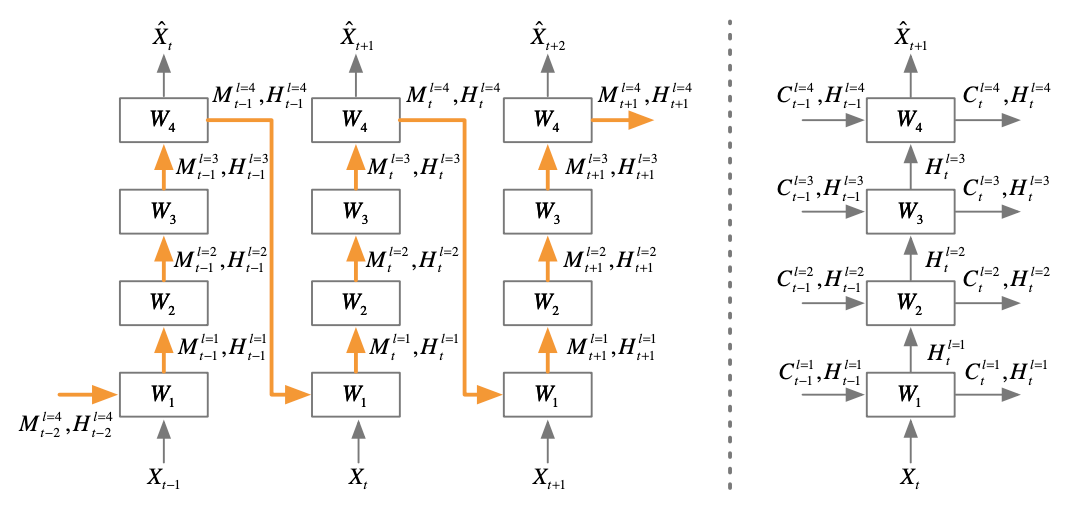
\includegraphics[width=\textwidth]{figures/videoprediction/predrnn_memory.png}
            \caption{左がPredRNNにおけ時空間メモリフロー、右がConvLSTMのメモリフローである。このような異なるレベルの層を通過するメモリフローにより、多様な抽象度の表現を学習することができる。}
            \label{fig:predrnn}
          \end{center}
        \end{figure}
        
        \subsubsection{時空間LSTMユニット (ST-LSTM)}
          時空間メモリフローは空間情報の効果的な伝達を可能にするが、水平方向(時間方向)のメモリフローを省略すると、時間的一貫性を犠牲にしてしまう。
          PredRNNでは、標準的なLSTMユニットを、時空間メモリセルとゲート構造を導入した時空間LSTM(ST-LSTM)ユニットに置き換える。
          ST-LSTMユニットは、時間メモリセルと時空間メモリセルの両方を維持し、それらを縦方向および横方向に流すことにより、一定の時間一貫性を担保しながら、異なる抽象度レベルでの特徴を捉える。
          また、ST-LSTMは1x1の畳み込み層を使用して次元削減を行い、隠れ状態の次元をメモリセルと同じにする。この構造により、PredRNNは時空間データの複雑なダイナミクスを捉え、より正確な予測を生成することができる。

          時空間LSTMの数学的定式化は以下の通りである。
          ここで、\( \ast \) は畳み込み演算を、\( \circ \) はアダマール積(要素ごとの積)を示す。
          \( W \) と \( b \) は重みとバイアスパラメータ、\( \sigma \) はシグモイド活性化関数、\( \tanh \) は双曲線正接活性化関数を指す。
          \( X_t \) は時刻 \( t \) の入力、\( H_t^l \) は隠れ状態、\( C_t^l \) は標準的なLSTMセル、\( M_t^l \) は時空間メモリセルを表す。
          \begin{align}
          g_t &= \tanh(W_{xg} \ast X_t + W_{hg} \ast H_{t-1}^l + b_g) \\
          i_t &= \sigma(W_{xi} \ast X_t + W_{hi} \ast H_{t-1}^l + W_{mi} \circ M_{t-1}^l + b_i) \\
          f_t &= \sigma(W_{xf} \ast X_t + W_{hf} \ast H_{t-1}^l + W_{mf} \circ M_{t-1}^l + b_f) \\
          C_t^l &= f_t \circ C_{t-1}^l + i_t \circ g_t \\
          g_t' &= \tanh(W_{xg}' \ast X_t + W_{mg} \ast M_{t-1}^l + b_g') \\
          i_t' &= \sigma(W_{xi}' \ast X_t + W_{mi} \ast M_{t-1}^l + b_i') \\
          f_t' &= \sigma(W_{xf}' \ast X_t + W_{mf} \ast M_{t-1}^l + b_f') \\
          M_t^l &= f_t' \circ M_{t-1}^l + i_t' \circ g_t' \\
          o_t &= \sigma(W_{xo} \ast X_t + W_{ho} \ast H_{t-1}^l + W_{co} \ast C_t^l + W_{mo} \ast M_t^l + b_o) \\
          H_t^l &= o_t \circ \tanh(W_{1 \times 1} \ast [C_t^l, M_t^l])
          \end{align}
          
          この構造により、PredRNNは時空間データの複雑なダイナミクスを捉え、より正確な未来予測を生成する。
          \begin{figure}[htbp]
            \begin{center}
              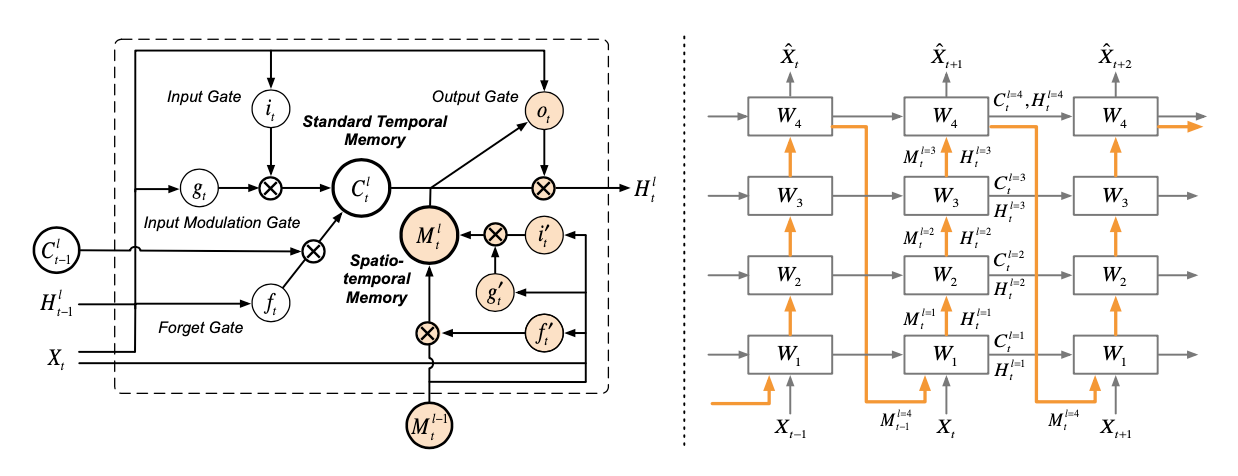
\includegraphics[width=160mm]{figures/videoprediction/predrnn_unit.png}
              \caption{左がST-LSTMユニット、右がPredRNNのメモリフロー。オレンジ色のノードは、従来のConvLSTMと異なるPredRNN独自の構造を示す。
              PredRNN内のオレンジ色の矢印は、時空間メモリ\( M_t^l \)の移行経路を示す。}
              \label{fig:stlstm}
            \end{center}
          \end{figure}
        
    \subsection{Motion-Aware Unit(MAU)}
      Motion-Aware Unit (MAU)は、\citex{chang2021mau}によって発表された、フレーム間のダイナミクスをより効率的に捉えるために提案された新しい動画予測アーキテクチャである。
      MAUは、PredRNNと似た積層LSTMの構造を持ち、そのLSTMユニットをMAUセルによって置き換えている。
      MAUセルは、注意(Attention)モジュールと融合(Fusion)モジュールの2つの部分から構成されており、PredRNNにおける時空間LSTMユニットをさらに拡張したものである。
      このような変更により、時間的受容野

      本研究では、このMAUを用いて太陽全球紫外線画像の予測を行う。
      
      \subsubsection{アーキテクチャ}
      動画予測モデルでは、出力中の時間ステップが進むほど、時間情報の不確実性が増加するため、予測誤差が劇的に加速してしまう。
      この問題を解決するため、動画予測モデルはより幅広い時間ステップから有用な特徴を保存し活用する必要がある。
      すなわち、時間的受容野を拡張する必要がある。
      このような問題に対するアプローチとして、\citex{wang2018eidetic}によって提案された、三次元畳み込みを導入したE3D-LSTMがあったが、非常に高い計算コストを必要とし、性能の改善は限定的であった。
      Motion-Aware Unit (MAU)は、このような課題を解決するため、Attention機構を導入した新しいアーキテクチャを提案している。
      ここでは、Attention機構を用いたアーキテクチャと、その統合や効率化のために導入されたいくつかの特徴について説明する。
      \begin{figure}[htbp]
        \begin{center}
          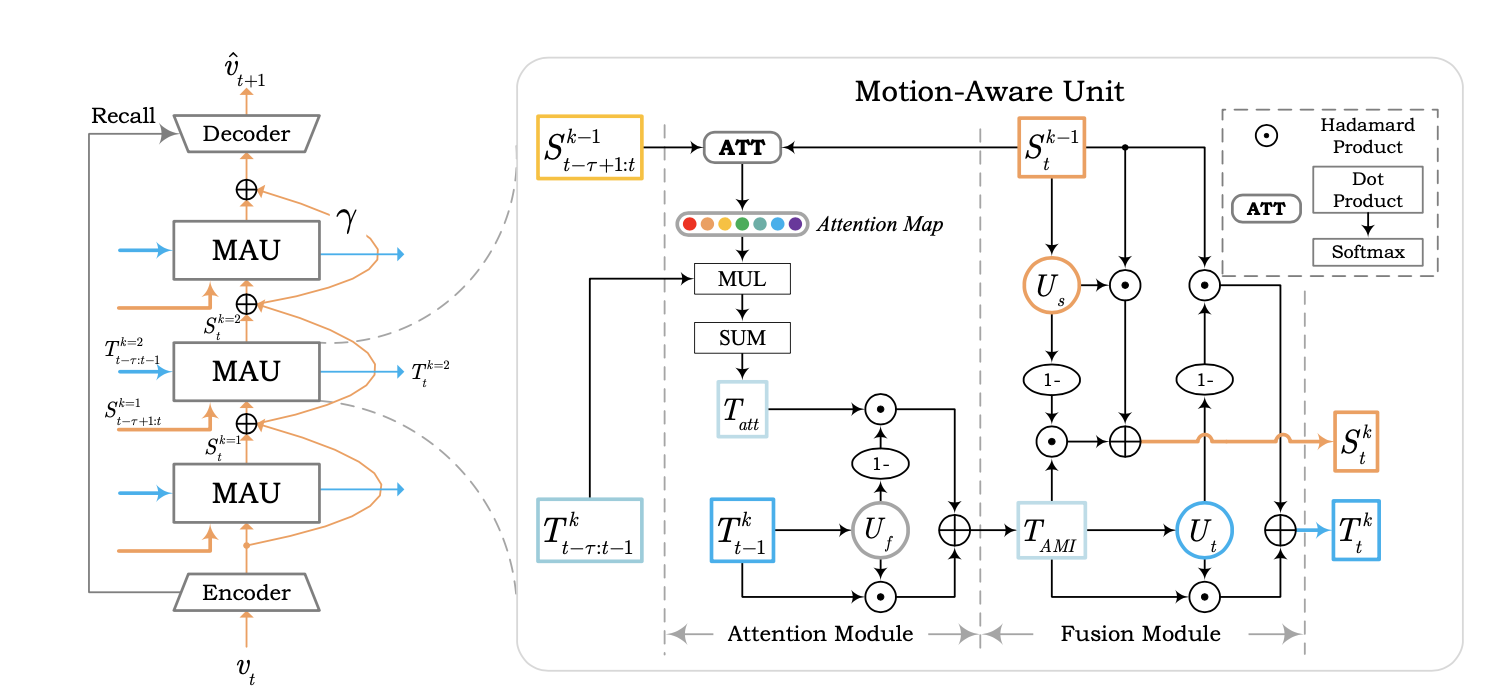
\includegraphics[width=160mm]{figures/videoprediction/mau.png}
          \caption{左: MAUセルを積み重ねたMAUモデルの構造。オレンジ色の矢印は空間方向のメモリフローを示し、青色の矢印は時間方向のメモリフローを示す。エンコーダ・デコーダ構造は各時間ステップにおいて一回ずつ適用され、情報を効果的に圧縮している。右:MAUセルは、注意(Attention)モジュールと融合(Fusion)モジュールの2つの部分から構成されている。}
          \label{fig:mau_attention}
        \end{center}
      \end{figure}
        
      \begin{itemize}

        \item \textbf{エンコーダ・デコーダ構造}: MAUは、エンコーダ・デコーダ構造を基本としている。
        Conv-LSTMやPred-RNNなどの他の動画予測モデルではエンコーダ・デコーダ構造は採用されていないが、MAUではエンコーダ・デコーダ構造を採用することで、より効率的な特徴抽出を可能にしている。
        一定程度抽象化された情報を再帰的ネットワークに入力することで、より多くのMAUセルの積層を行っても、計算コストを抑えることができる。
        \begin{align}
          \hat{X}_t &= \text{Dec}[\text{MAU}(\text{Enc}(X_{t-\tau:t-1}))]
        \end{align}
        ここで、\( \text{Enc} \) はエンコーダ、\( \text{Dec} \) はデコーダを表し、\( \tau \) は入力シーケンスの長さを表す。
          
        \item \textbf{注意(Attention) モジュール}: 
        注意モジュールは、先述の時間的受容野の拡張のために導入される。
        このモジュールの導入により、異なる時間状態に対して異なるレベルの注意を払い、予測に対してもっとも相関の高い状態に注意を集中させることが期待されている。
        長期的な運動情報としての\( T_{\text{att}} \)は以下のように計算される。
        \begin{align}
          T_{\text{att}} = \sum_{j=1}^{\tau} \alpha_j \cdot T_{t-j}^{k}
        \end{align}
        ここで、\( \alpha_j \) は時間状態\( T_{t-j}^{k} \)に対するアテンションスコアを表す。
        \( T_{\text{att}} \) は、アテンションスコアによって、予測結果に対して長期的な相関性を持つ時間状態を考慮することができるが、短期的な時間状態 \( T_{t-1}^{k} \) も考慮する必要がある。
        そこで、それらを融合するためのゲート \( U_f \) を導入し、長期的な時間状態 \( T_{\text{att}} \) と短期的な時間状態 \( T_{t-1}^{k} \) を融合した\( T_{AMI} \)を以下のように計算する。
        \begin{align}
          U_f = \sigma(W_f \ast T_{t-k-1}) \\
          T_{AMI} = U_f \odot T_{t-k-1} + (1 - U_f) \odot T_{\text{att}} 
        \end{align}

        \item \textbf{融合(Fusion) モジュール}: 融合モジュールは、拡張された運動情報\(T_{\text{AMI}} \)と現在の空間的状態を適切に統合する役割を持つ。融合プロセスでは、時間的更新ゲート\( U_t \)と空間的更新ゲート\( U_s \)を導入する。
        \begin{align}
          U_t = \sigma(W_{\text{tu}} \ast T_{\text{AMI}}) \\
          U_s = \sigma(W_{\text{su}} \ast X_t) 
        \end{align}
        ここで、\( W_{\text{tu}} \) と \( W_{\text{su}} \) はそれぞれ時間的更新ゲートと空間的更新ゲートの重みを表す。
        このゲートを利用して、時間状態\( T_{t}^{k} \)と空間状態\( S_{t}^{k} \)を以下のように計算する。
        \begin{align}
        T_{t}^{k} = U_t \odot (W_{tt} \ast T_{\text{AMI}}) + (1 - U_t) \odot (W_{st} \ast S_{t}^{k-1}) \\
        S_{t}^{k} = U_s \odot (W_{ss} \ast S_{t}^{k-1}) + (1 - U_s) \odot (W_{ts} \ast T_{\text{AMI}}) + \gamma \cdot S_{t}^{k-1}
        \end{align}
        ここで、\( W_{tt} \)、\( W_{st} \)、\( W_{ss} \)、\( W_{ts} \) はそれぞれ時間状態と空間状態の重みを表し、\( \gamma \) は学習の安定化を図るための残差項の係数である。

        \item \textbf{情報リコール}: 
          MAUでは、エンコーダとデコーダ間で情報損失を防ぐために、情報リコールスキームが採用されている。これはU-Netなどでで用いられるスキップ接続に似た構造を持っている。これにより、デコーダは多レベルのエンコードされた情報を考慮することができ、予測の視覚的品質を向上させることができる。    

       \end{itemize}

      \subsubsection{主な実験結果}
        MAUは、複数のデータセットで評価され、その中にはMoving MNIST、KITTI、Caltech Pedestrian、TownCentreXVID、Something-Something V2が含まれる。
        ここでは、Moving MNISTデータセットに関する既存の動画予測モデルによる性能との比較の結果を示す。
        表\ref{mau-mnist-1}は、異なる手法によるMoving MNISTデータセットにおける定量的な結果を示している。
        MAUは、構造的類似性(Structual Similarity, SSIM)スコアと平均二乗誤差(Mean Squared Error, MSE)スコアの両方において、最も優れた結果を示している。
        \ref{mau-mnist-2}は、LSTMユニットを積層する動画予測モデルのバックボーンを統一し、それぞれの場合でのパラメータと推論時間に焦点を当てた比較を行なっている。
        これによれば、MAUは他の手法と比較して、より少ないパラメータ数とより短い推論時間で動作することができ、さらにMSEとSSIMの両方において最も優れた結果を示している。

        \begin{table}[hptb]
          \centering
          \caption{Moving MNISTデータセットにおけるビデオ予測方法の定量的結果(10フレーム→10フレーム)。低いMSEと高いSSIMスコアはより良い視覚的品質を示す。}
          \label{mau-mnist-1}
          \begin{tabular}{lcc}
          \hline
          \textbf{方法} & \textbf{SSIM/frame$\uparrow$} & \textbf{MSE/frame$\downarrow$} \\ \hline
          ConvLSTM (NeurIPS2015) & 0.707 & 103.3 \\
          FRNN (ECCV2018)  & 0.819 & 68.4 \\
          VPN (ICML2017) & 0.870 & 70.0 \\
          PredRNN (NeurIPS2017) & 0.869 & 56.8 \\
          PredRNN++ (ICML2018) & 0.898 & 46.5 \\
          MIM (CVPR2019) & 0.910 & 44.2 \\
          E3D-LSTM (ICLR2019) & 0.910 & 41.3 \\
          CrevNet (ICLR2020) & 0.928 & 38.5 \\
          MAU (w/o recalling) & 0.931 & 29.5 \\
          MAU & \textbf{0.937} & \textbf{27.6} \\ \hline
          \end{tabular}
        \end{table}
          
        \begin{table}[hptb]
          \centering
          \caption{Moving MNISTデータセット(10フレーム→10フレーム)に対する比較。公平な比較のため、すべてのモデルのエンコーダとデコーダは同じ構造をしており、すべてのモデルはMSE損失に基づいてAdamオプティマイザーを用いて訓練されている。}
          \label{mau-mnist-2}
          \begin{tabular}{lccccc}
          \hline
          \textbf{方法}            & \textbf{バックボーン} & \textbf{MSE$\downarrow$} & \textbf{SSIM$\uparrow$} & \textbf{パラメータ数} & \textbf{推論時間} \\ \hline
          ConvLSTM (NeurIPS2015) & 4×ConvLSTMs   & 102.1  & 0.747  & 0.98M   & 16.47s \\
          ST-LSTM (NeurIPS2017)  & 4×ST-LSTMs    & 54.5   & 0.839  & 1.57M   & 17.74s \\
          Casual-LSTM (ICML2018) & 4×Casual-LSTMs & 46.3   & 0.899  & 1.80M   & 21.25s \\
          MIM (CVPR2019)     & 4×MIMs        & 44.1   & 0.910  & 3.03M   & 45.13s \\
          E3D-LSTM (ICLR2019) & 4×E3D-LSTMs   & 40.1   & 0.912  & 4.70M   & 57.21s \\
          RPM (ICLR2020)     & 4×RPMs        & 42.0   & 0.922  & 1.77M   & 18.01s \\
          MotionGRU (CVPR2021)& 4×MotionGRUs  & 34.3   & 0.928  & 1.16M   & 17.58s \\
          MAU                 & 4×MAUs        & \textbf{29.5}   & \textbf{0.931}  & \textbf{0.78M}   & \textbf{17.34s} \\ \hline
          \end{tabular}
        \end{table}
\chapter{データ} 

\section{SDO / AIA}
モデルの学習及び評価データとして、NASAのSolar Dynamic Observatory(SDO)(\cite{pesnell2012solar})のAtmospheric Imaging Assembly(AIA)(\cite{lemen2012atmospheric})で撮影された紫外線観測データを用いた。

SDOはNASAのLiving With a Star(LWS)プログラムの一つとして2010年2月に打ち上げられた太陽観測衛星である。
AIA、Helioseismic and Magnetic Imager(HMI)、Extreme Ultraviolet Variability Experiment(EVE)などの高い空間解像度、時間分解能を持つ観測機器を搭載し、地上では不可能な多くの波長でのデータを提供する。
その観測データを用いることにより、太陽物理学、宇宙天気、また地球環境に関する理解や洞察を深めることが期待されている。

AIAは主に太陽大気を観測する観測機器であり、4つの望遠鏡で構成されている。
また、7つの極紫外線フィルターと、2つの紫外線フィルター、および1つの可視光フィルターを持ち、広範な温度帯で太陽大気を観察することを可能にしている。
本研究で用いられる171Å、193Å、211Åの3つのフィルターは、36秒間隔で撮影され、4096×4096、約1.5秒角の空間解像度を持つ

これらのデータはJoint Science Operations Center(JSOC) によって提供されており、Pythonの太陽物理学を支援するライブラリであるSunpyを用いてダウンロードすることができる。


\subsection{AIA 211Å}
    表\ref{table:aia_filters_details}のように、211Å( 21.1 nm )のフィルターは、約200万Kの14価鉄(Fe XIV)イオンが放射するスペクトルを捉えるために特化している。
    この波長での観測は、活動領域のコロナを観測するのに最適である。図\ref{fig:sample_aia211}は、これらの特性を示している。

    \begin{figure}[h]
        \centering
        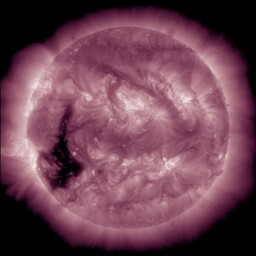
\includegraphics[width=0.8\textwidth]{figures/data/latest_256_0211.jpg}
        \caption{SDO/AIAの211Åフィルターで撮影された太陽全球紫外線像。強調のために紫色に色付けされている。球面の中上部から中下部には明るく輝く活動領域が見られ、左下部に暗くコロナホールが観測できる。}
        \label{fig:sample_aia211}
    \end{figure}

\subsection{AIA 193Å}
    表\ref{table:aia_filters_details}のように、193Å( 19.3 nm )のフィルターは、約150万Kの12価鉄(Fe XII)イオンが放射するスペクトル、または約2000万Kの24価鉄(Fe XXIV)イオンが放射するスペクトルを捉えるために特化している。
    前者は主にコロナの中程度の高温領域を観測するために用いられ、後者は、主にコロナの高温フレアプラズマを観測するために用いられる。さらに、コロナホールも強調して観測することができる。
    図\ref{fig:sample_aia193}は193Åフィルターで捉えた太陽像を示している。
    
    \begin{figure}[h]
        \centering
        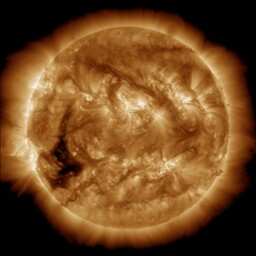
\includegraphics[width=0.8\textwidth]{figures/data/latest_256_0193.jpg}
        \caption{SDO/AIAの193Åフィルターで撮影された太陽全球紫外線像。強調のために橙色に色付けされている。}
        \label{fig:sample_aia193}
    \end{figure}
    
\subsection{AIA 171Å}
    表\ref{table:aia_filters_details}のように、171Å( 17.1 nm )のフィルターは、約60万Kの9価鉄(Fe IX)イオンが放射するスペクトルを捉えるために特化している。
    この波長での観測は、太陽のコロナループ、静穏領域コロナ、コロナホールなどの磁気構造を詳細に観察することができる。
    図\ref{fig:sample_aia171}に示される171Åフィルターによる観測は、これらの特徴を捉えている。
    
    \begin{figure}[h]
        \centering
        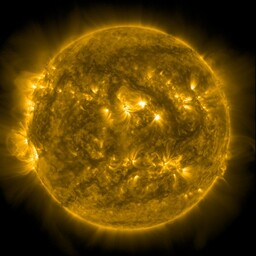
\includegraphics[width=0.8\textwidth]{figures/data/latest_256_0171.jpg}
        \caption{SDO/AIAの171Åフィルターで撮影された太陽全球紫外線像。強調のために黄色に色付けされている。193Å、211Åでは観察できない、コロナホールなどの静穏領域のスペクトルも観測できる。}
        \label{fig:sample_aia171}
    \end{figure}

\begin{table}[hptb]
    \centering
    \caption{SDO AIAの171, 193, 211(\AA)の特性}
    \begin{tabular}{lccc}
    \hline
    \textbf{フィルター (\AA)} & \textbf{主要イオン} & \textbf{大気の領域} & \textbf{温度帯(K)}  \\ \hline
    171 & Fe IX & 静穏領域コロナ, 上層遷移領域 & \(6.3 \times 10^{5} \) \\ \hline
    193 & Fe XII, XXIV & コロナと高温フレアプラズマ & \(1.5 \times 10^6, 2.0 \times 10^7 \)  \\ \hline
    211 & Fe XIV & 活動領域コロナ & \(2.0 \times 10^6\) \\ \hline
    \end{tabular}
    \label{table:aia_filters_details}
\end{table}


\section{前処理}

本研究で用いるデータセットには、SDO/AIAのデータが提供されている2010年5月から、2022年10月までのデータが含まれている。  
この期間に存在するデータから、4時間ごとにデータを抽出し、各波長ごとに約22000枚をデータセットに含んでいる。
データはJSOCにより提供されているものをダウンロードし、その後、不正な画像を除去し、正規化やスケーリングを行った後、学習用、検証用、テスト用に分割した。
この手順をアルゴリズム\ref{alg:dataset_creation}に示す。
これらのデータを、24枚の画像を1セットとして分割する。各セットは24枚の時系列に並んだ画像で構成され、太陽全球の空間的情報の時間的変化を捉えている。
24枚のうち、前半の12枚、すなわち48時間までを入力シークエンス 、後半の12枚、すなわち52時間から96時間までを出力シークエンスとして扱う。
学習の際は、入力シークエンスに対して出力シークエンスを教師データとして扱い、テストの際は入力シークエンスに続くモデルにとって未知の出力シークエンスを再現できるか検証する。

このデータセットは第24太陽活動周期の初期から、第25周期の初期までの観測データを網羅している。この時間範囲には、太陽活動の活発性が高いフェーズと低いフェーズの両方が含まれている。従って、このデータセットは太陽活動の活発性に依存しない可能性が高く、その汎化能力に対する期待が一定程度裏付けられる。

\begin{algorithm}
    \caption{データセット作成アルゴリズム}
    \label{alg:dataset_creation}
    \begin{algorithmic}[1]
    \Procedure{CreateSolarDataset}{}
        \For{each wavelength in wavelengths}
            \State $images \gets \Call{DownloadData}{wavelength}$
            \State $images \gets \Call{ValidateAndReplaceImages}{images}$
            \State $all\_images.extend(images)$
        \EndFor
        \State $dataset \gets \Call{CreateDataset}{all\_images}$
        \State $processed\_dataset \gets \Call{PreprocessDataset}{dataset}$
        \State $train, val, test \gets \Call{SplitDataset}{processed\_dataset}$
        \State \Return $train, val, test$
    \EndProcedure
    
    \Function{DownloadData}{wavelength}
        \State \textit{Download data for given wavelength}
        \State \Return $images$
    \EndFunction
    
    \Function{ValidateAndReplaceImages}{images}
        \For{each image in images}
            \If{\textbf{not} \Call{ValidateImage}{image}}
                \State $alternative \gets \Call{FindAlternativeImage}{image.timestamp}$
                \State $images.replace(image, alternative)$
                \State \Call{ValidateAndReplaceImages}{images} \Comment{Recursive call}
            \EndIf
        \EndFor
        \State \Return $images$
    \EndFunction
    
    \Function{CreateDataset}{images}
        \State \textit{Create dataset by grouping 24 images}
        \State \Return $dataset$
    \EndFunction
    
    \Function{PreprocessDataset}{dataset}
        \State \textit{Apply preprocessing to each image in dataset}
        \State \Return $processed\_dataset$
    \EndFunction
    
    \Function{SplitDataset}{dataset}
        \State \textit{Split the dataset into train, validation, and test sets}
        \State \Return $train, val, test$
    \EndFunction
    \end{algorithmic}
\end{algorithm}

\subsection{不正な画像の除去}
SDO/AIA望遠鏡で撮影された全球画像には、露光時間が他の画像より極端に低い、画像内に太陽全体を捉えていない、などの不正な画像が含まれている。
確認することができた主な不正な画像を図\ref{fig:bad_aia_samples}に示す。

\begin{figure}[htbp]
    \centering
    \begin{subfigure}[b]{0.48\textwidth}
        
\includegraphics[width=\textwidth]{figures/data/bad_sample0.png}
        \caption{短い露光時間により、極端に暗い画像。}
    \end {subfigure}
    \hfill
    \begin{subfigure}[b]{0.48\textwidth}
        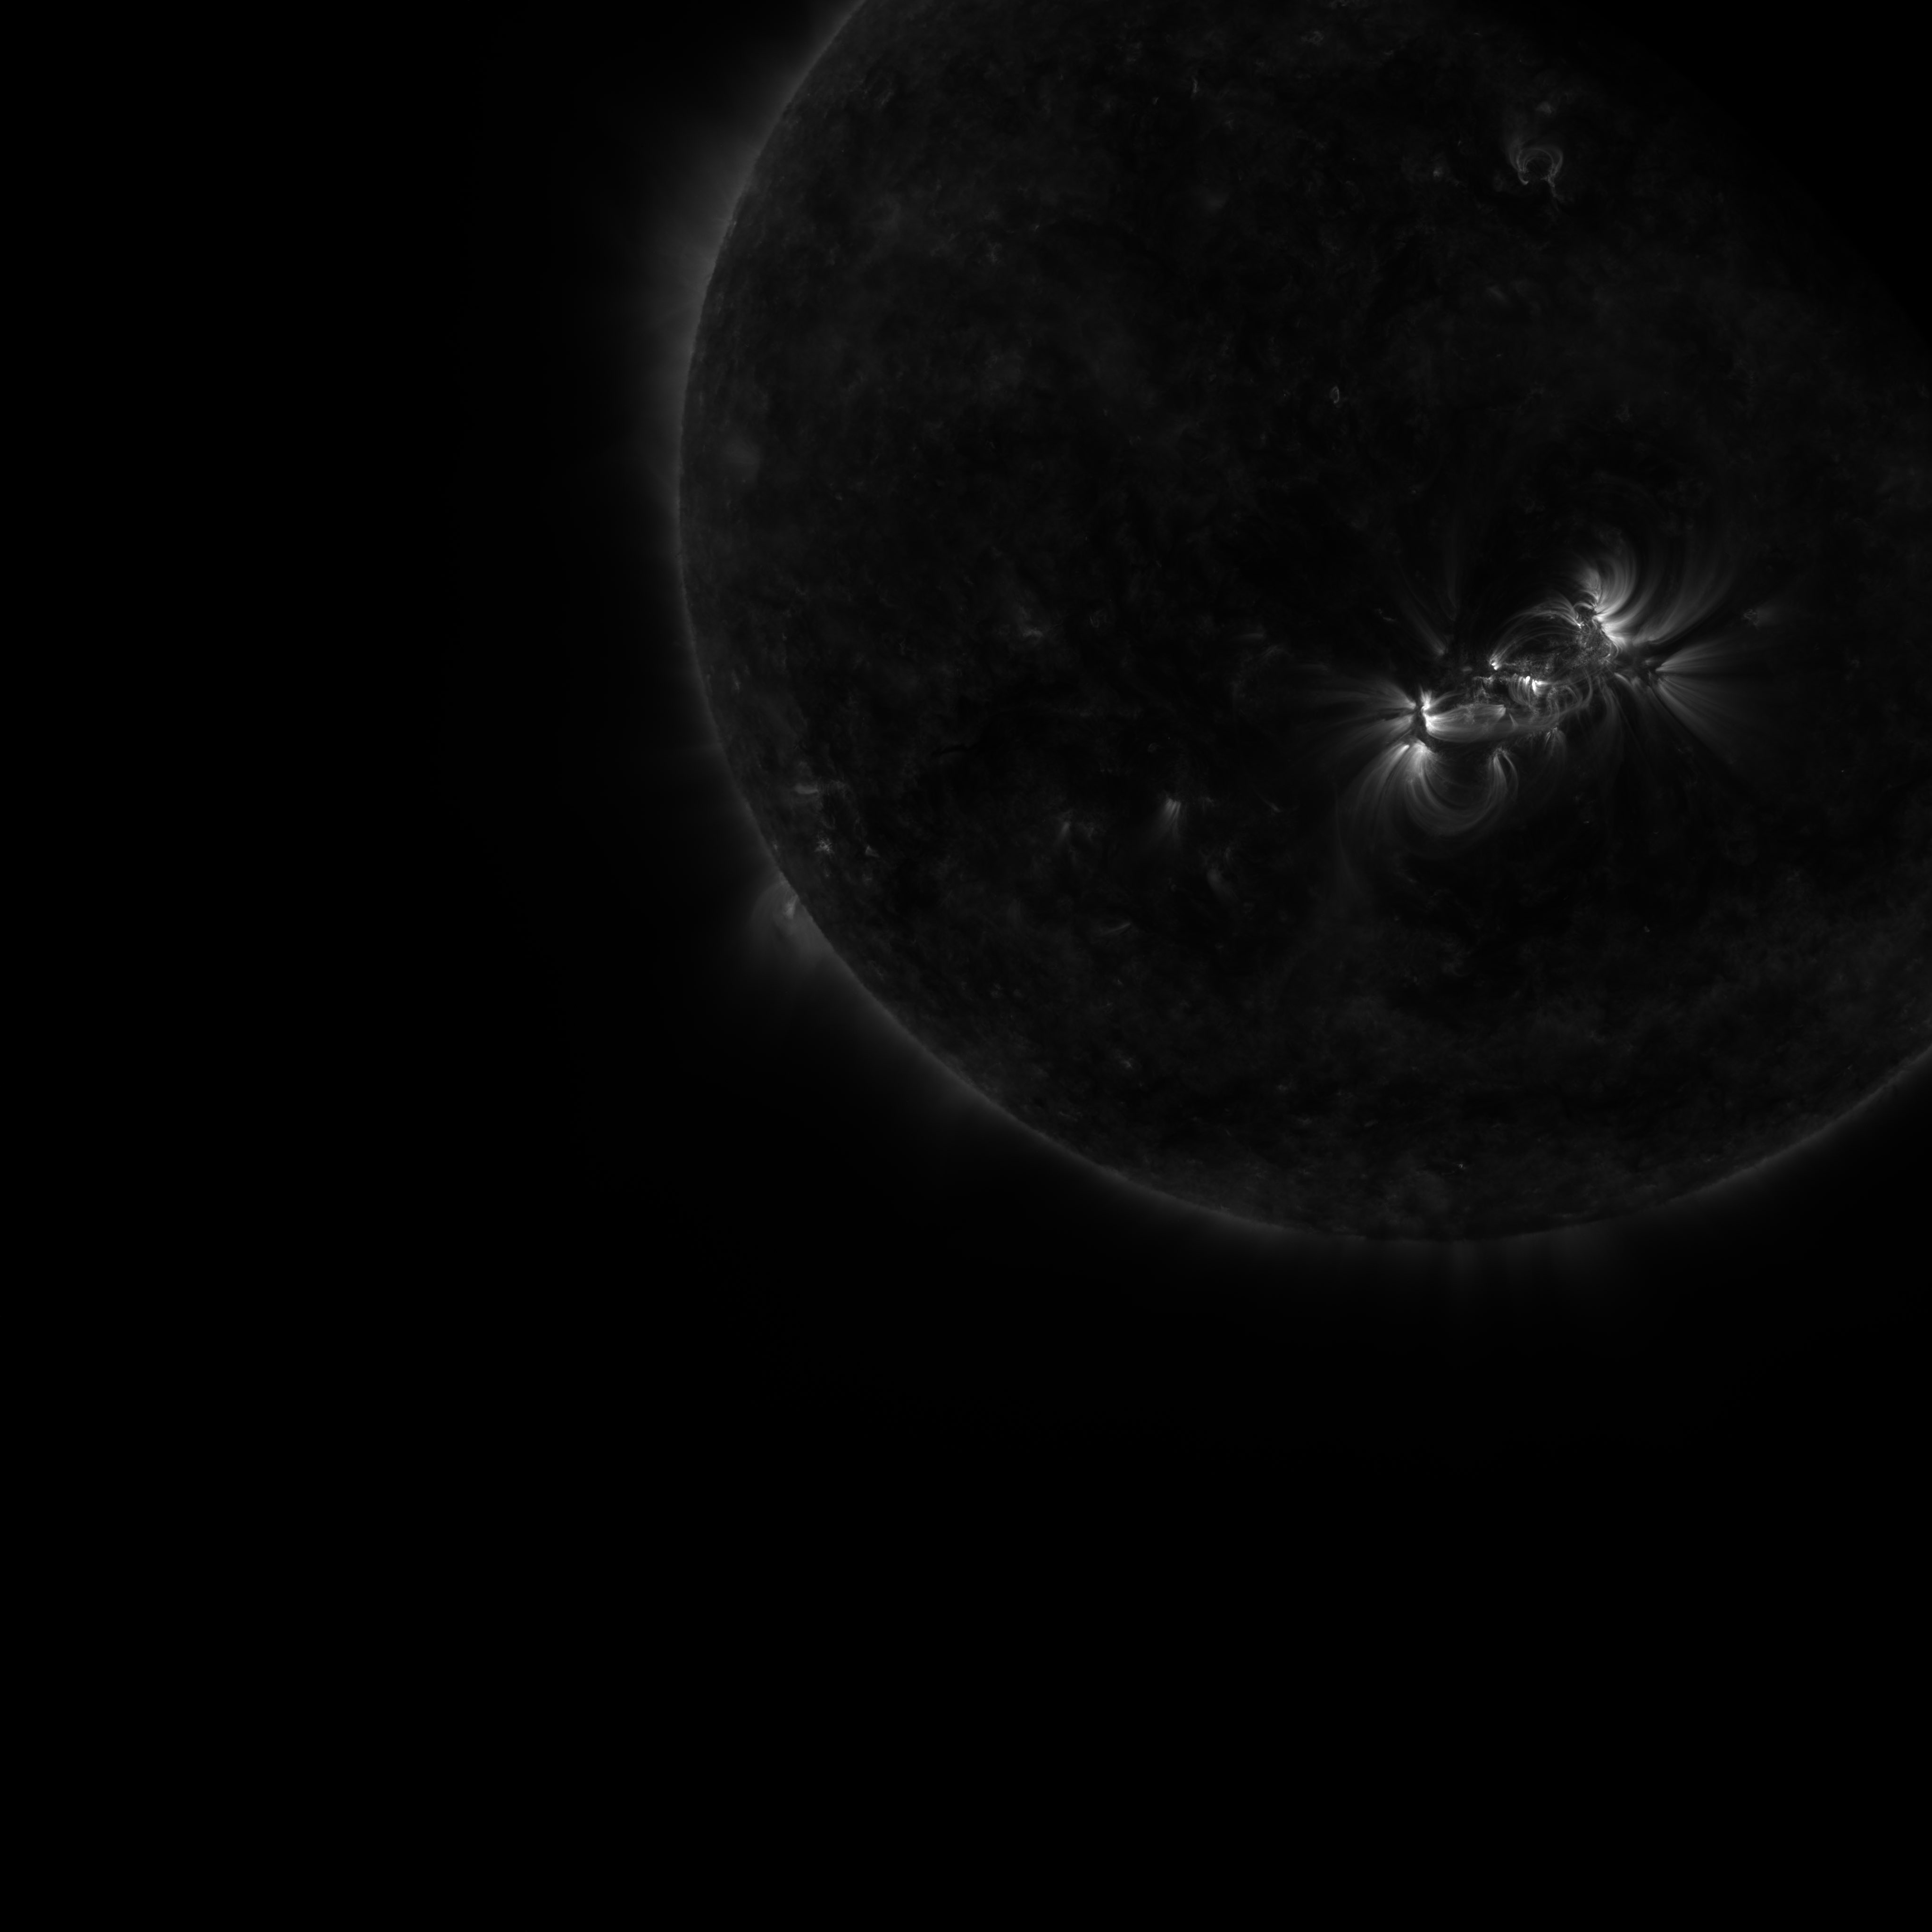
\includegraphics[width=\textwidth]{figures/data/bad_sample1.jpg}
        \caption{太陽が画像の中心にない画像。}
    \end {subfigure}
    \begin{subfigure}[b]{0.48\textwidth}
        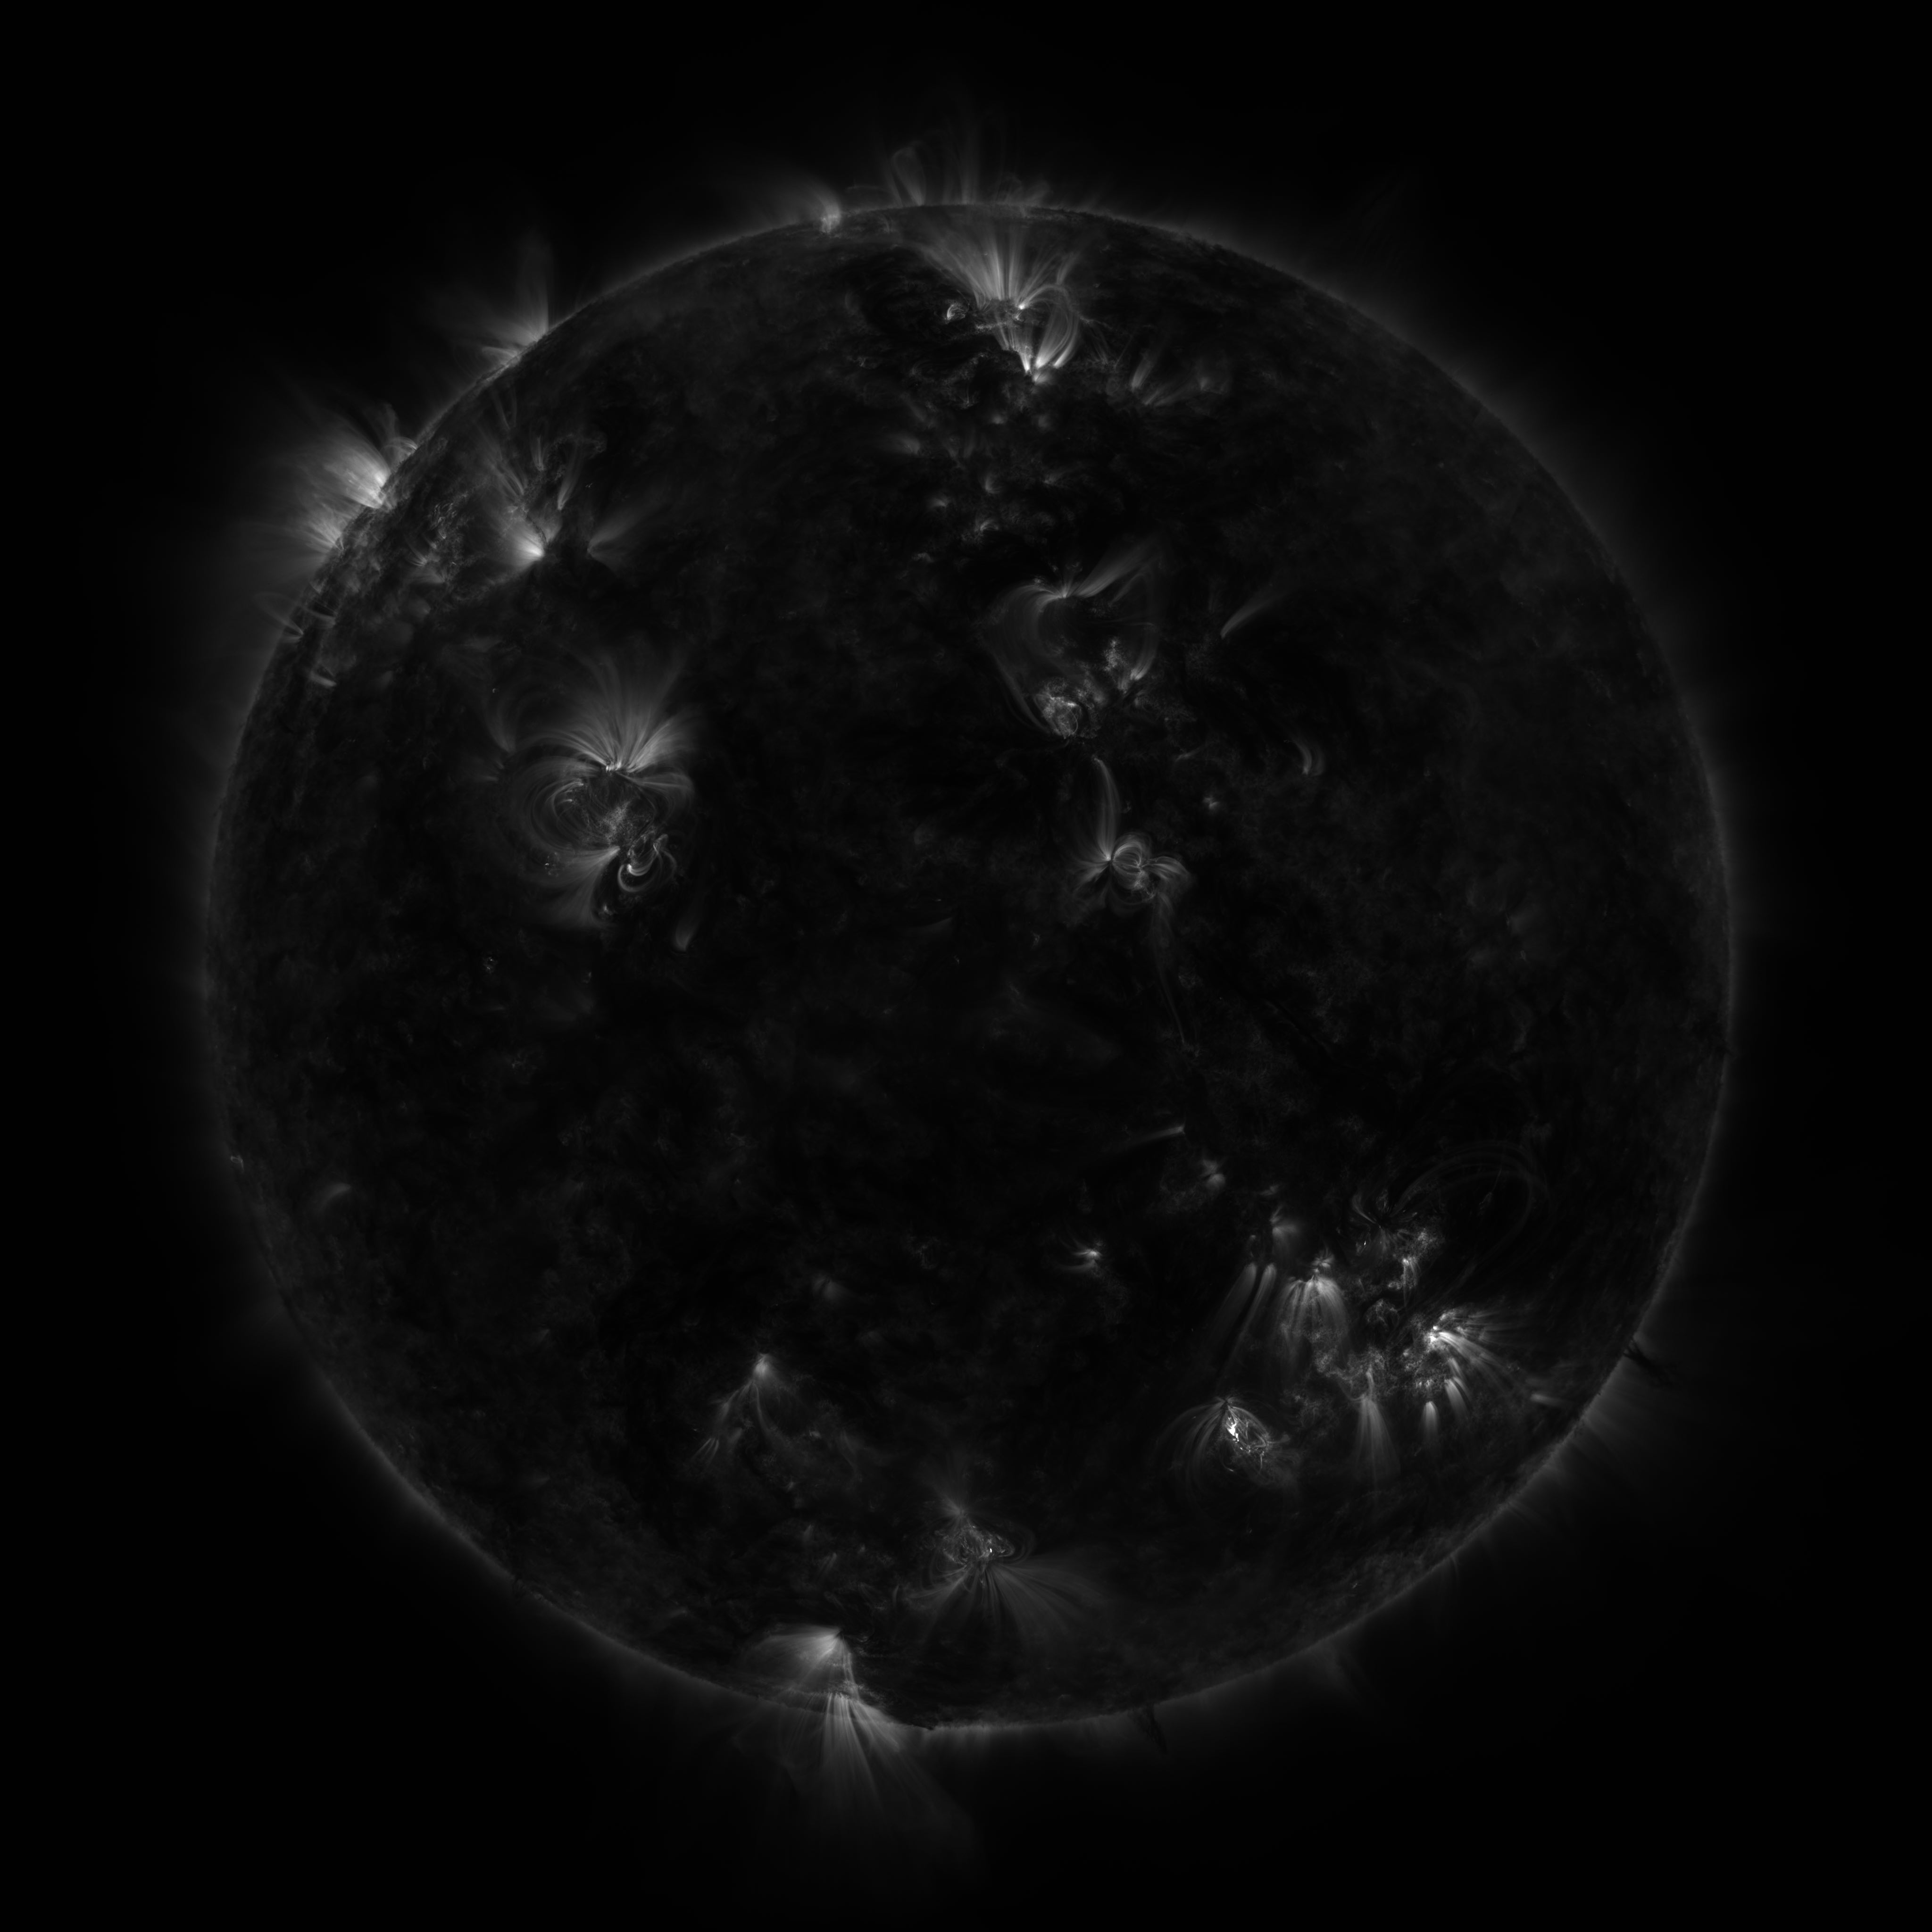
\includegraphics[width=\textwidth]{figures/data/bad_sample2.jpg}
        \caption{衛星が回転しており、正しい角度で太陽が撮影されていない画像。活動領域の少ない左下部と右上部が極である。}
    \end {subfigure}
    \hfill
    \caption{SDO/AIAにより観測された不正な画像の例}
    \label{fig:bad_aia_samples}
\end{figure}

これらの画像は、モデルの学習に悪影響を及ぼす可能性があるため、データセットから除去した。
機械学習のタスクによっては、十分なデータセットがあれば、モデルが不正な画像に対する頑健性を獲得し、不正な画像がデータセットに含まれていても、学習結果にあまり大きな影響を与えない場合がある。
しかし、本研究で行う動画予測は、データセットに含まれる画像がそのまま教師データとなるため、不正な画像は損失関数の計算、またはモデルの評価に大きな影響を与えるため、慎重に除去する必要がある。
データの除去には、FITSファイルのヘッダーに記録された各キーワードの値に対して閾値を設定して判定したのち、numpyによる輪郭検出を用いた月蝕判定関数により不正な画像を排除した。

\subsection{スケーリングと正規化}
    太陽動画データセットの前処理として、以下のステップを実施する。

    1. \textbf{正規化}: クリッピング処理されたデータを0から1の範囲に正規化する。ここで、ノイズによる負の値を削除し、極端に大きい外れ値の影響を削減するために、画像内の全ピクセル値に対して最小値を0、最大値を10000に設定した:
       \begin{equation}
       I_{normalized}(x, y) = \frac{min(max(I(x,y), 0), 10000)}{10000}
       \end{equation}

    2. \textbf{平方根スケーリング}: ダイナミックレンジの広さに対応するために、正規化されたデータに平方根スケーリングを適用する。この過程は以下の式で示される。
       \begin{equation}
       I_{scaled}(x, y) = \sqrt{I_{normalized}(x, y)}
       \end{equation}
        図\ref{fig:scale_histogram}のヒストグラムに示すように、スケーリングが適用されていないデータ(左)は、下位5\%程度の範囲に極端に輝度が集中している。平方根スケーリングを適用したデータ(右)では、そのような極端な輝度の差が緩和されている。

    \begin{figure}[htbp]
        \centering
        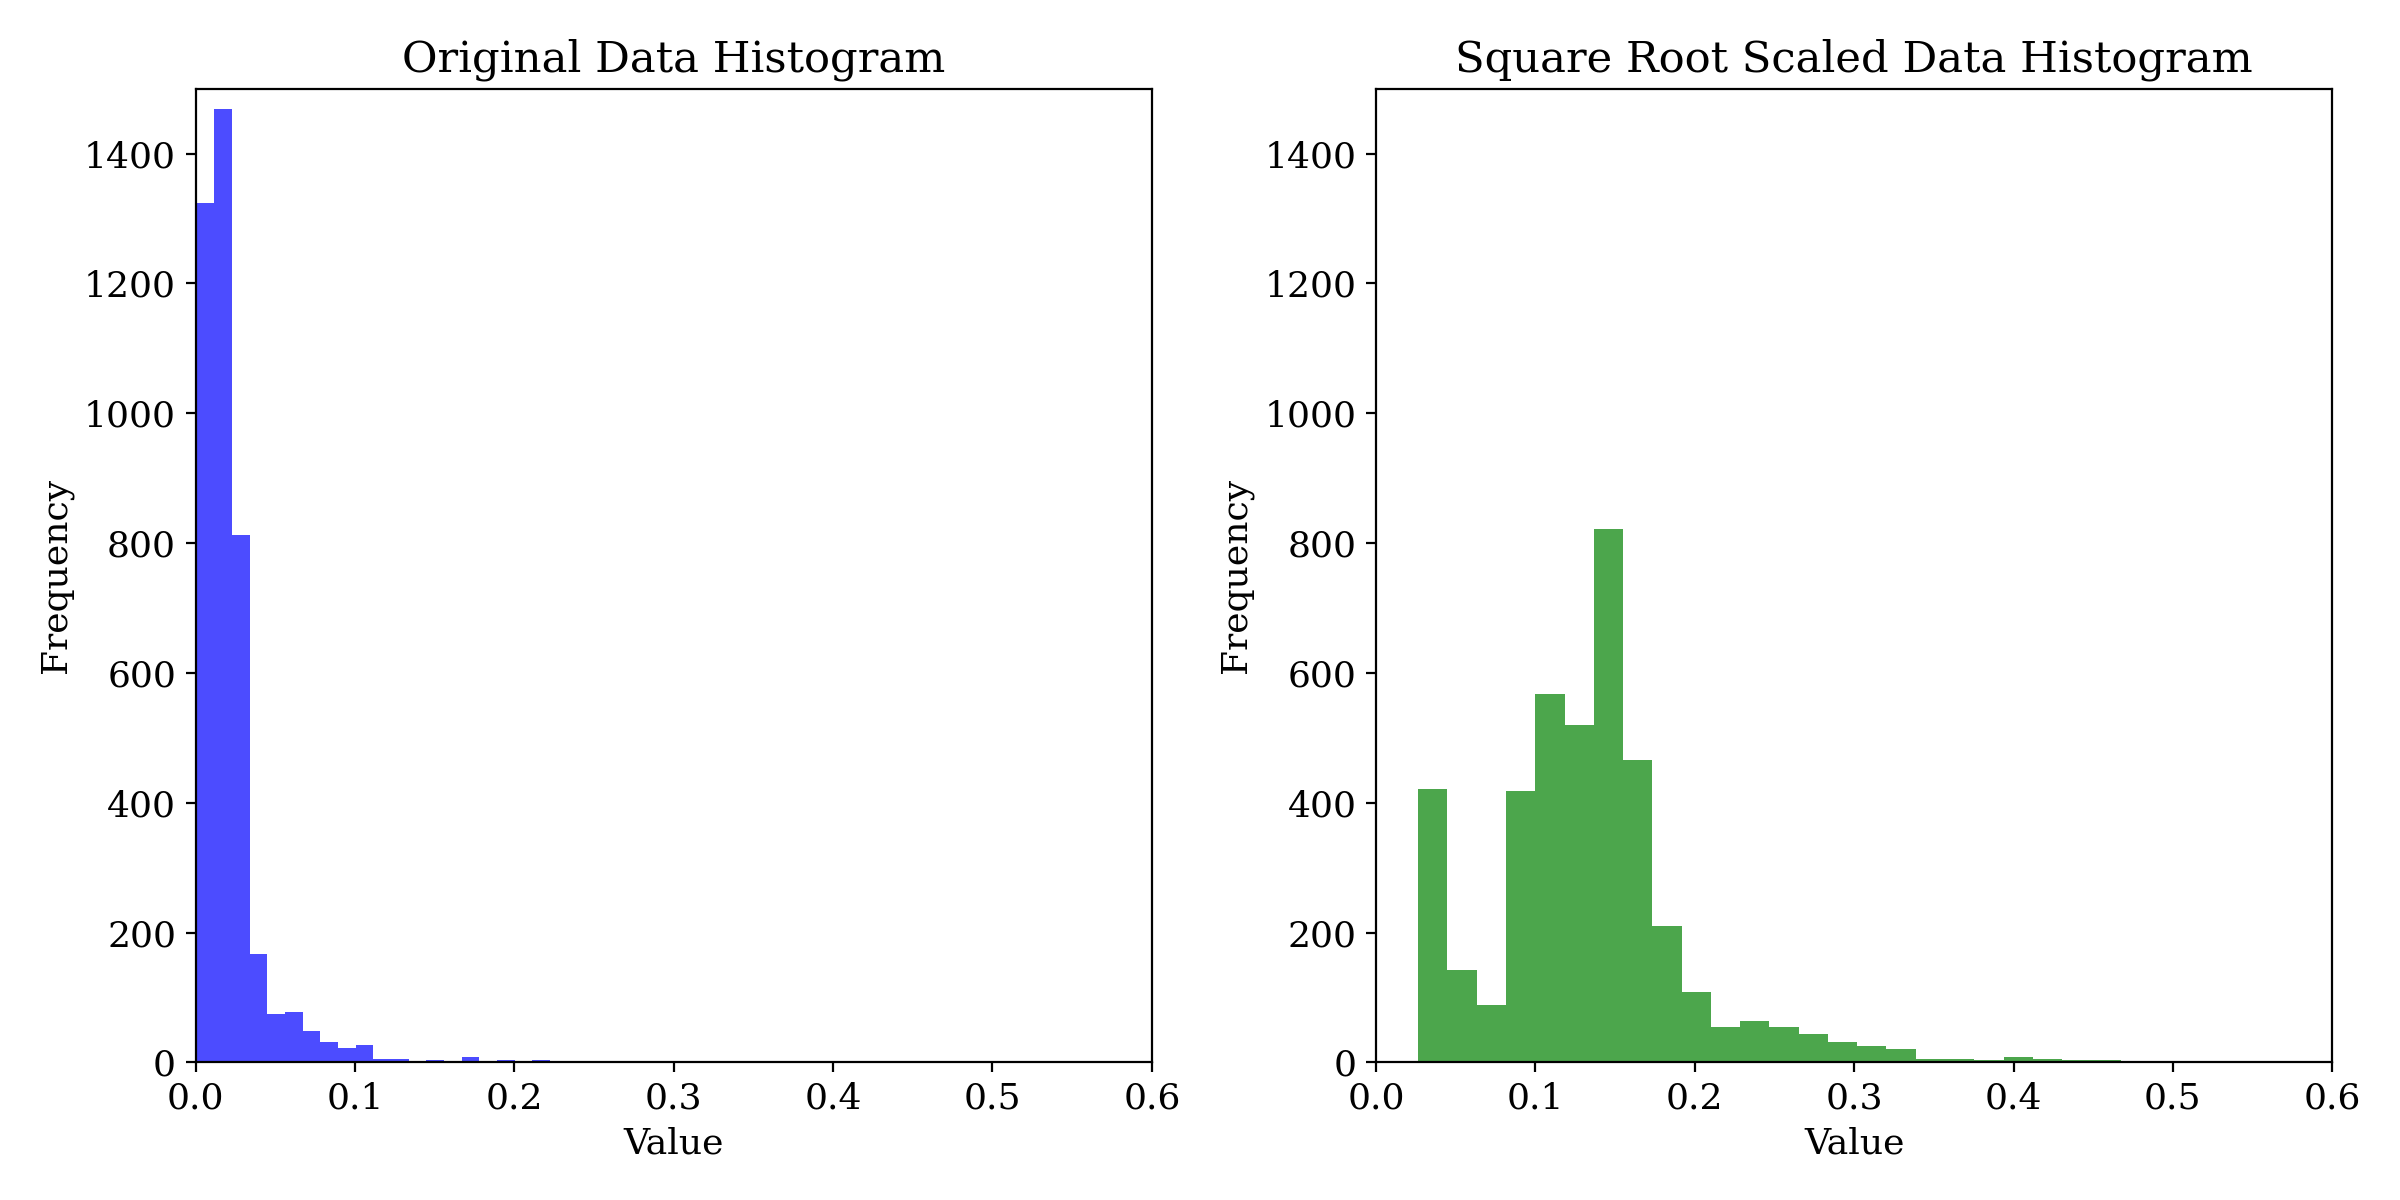
\includegraphics[width=\linewidth]{figures/data/histogram.png}
        \caption{ある画像での正規化されたデータに対する平方根スケーリングの効果。左: 正規化されたデータのヒストグラム。右: 平方根スケーリングを適用したデータのヒストグラム。}
        \label{fig:scale_histogram}
    \end{figure}

    3. \textbf{リサイズ}: 効率的な処理のために、$4192\text{px} \times 4192\text{px}$ の画像を$512\text{px} \times 512\text{px}$の解像度にリサイズした。この処理は、画像の空間解像度を低下させるが、太陽全球の大規模な構造を捉えるには十分である。


\subsection{データセットの分割}
このようにして作成されたデータセットは、約1000セットになり、これを学習用データセットに約800セット、検証データセットに50セット,テストデータセットに50セットというように分割した。
データセット1単位は、24枚の画像から構成される。

実験1では、211Åフィルターの画像のみを用いた。実験2では、171Å、193Å、211Åの3つのフィルターの画像を用いた。
最終的な分割とデータセットの概要を表\ref{tab:dataset}に示す。

\begin{table}[h]
    \centering
    \begin{tabular}{l|c|c}
    \hline
    実験 & 実験1 & 実験2 \\
    \hline\hline
    入力波長 & 211Å & 171Å,193Å,211Å \\
    \hline
    出力波長 & \multicolumn{2}{c}{211Å} \\
    \hline
    総枚数 & 22000 & 66000 \\
    \hline
    セット数 & \multicolumn{2}{c}{約1000} \\
    \hline
    セットごとの枚数 & \multicolumn{2}{c}{入力12 → 出力12} \\
    \hline
    解像度 & \multicolumn{2}{c}{512 * 512} \\
    \hline
    \end{tabular}
    \caption{各実験でのデータセット}
    \label{tab:dataset}
\end{table}





\chapter{Motion Aware Unitを用いた1波長を入力とした紫外線像の全球時系列予測}
  \section{実験概要}
  実験1では入力、出力ともに211Åフィルターで得られたデータを利用した。これは 211Åフィルターで撮影された紫外線像が、コロナホールと活動領域といった、二つの太陽円盤上の大規模構造をバランスよく明瞭に表現し、本研究のモデルの効果検証に適していると考えたためである。
  \section{学習の推移}
  \section{実験結果}
    \subsection{全球での評価}
      \subsubsection{平均輝度とその誤差}
      \subsubsection{画像類似度}
      \subsubsection{単純差動回転モデルとの比較}
      \subsection{経度依存性の評価}
        \subsubsection{平均輝度とその誤差}
        \subsubsection{単純差動回転モデルとの比較}
    \subsection{東側リムから出現する活動領域に対する視覚的評価}
  \section{考察}

\chapter{Motion-Aware Unitを用いた3波長を入力とした紫外線像の全球時系列予測}
  \section{実験概要}
    ここでは、171Å、193Åフィルターで得られたデータを追加で利用し、3波長の入力データから211Åの波長データに対する予測を行った。
    これらの波長は、太陽のコロナ領域における異なる温度帯を観測するためのものであり、予測モデルに多様な物理的情報を提供することが期待される。
    171Åの波長は、太陽のコロナにおける温度が約60万Kの領域を捉えるのに特化しており、193Åの波長は約100万Kの領域を捉える。
    これらの波長から得られる情報を組み合わせることにより、単一の波長では捉えられない層間の相互作用を捉え、より高い精度での予測を可能にすることを期待する。
    
    モデルには先の実験と同じく、MAUを用いる。入力は3波長、すなわち画像的には3チャンネルである。
    目的となる出力は211Åの波長のみであるが、MAUは3チャンネルを出力する。
    これは、「出力シークエンスのタイムステップ1以降では、直前のモデルの出力を入力データとして扱う」という動画予測モデルの一般的な性質によるものである。
    このような性質から、211Åの波長のみを出力として扱うために、出力された3チャンネルのうち、211Åの波長のみを抽出するという処理を行った
    図\ref{fig:exp2_concept}に本実験の概念図を示す。
    \begin{figure}[htbp]
      \centering
      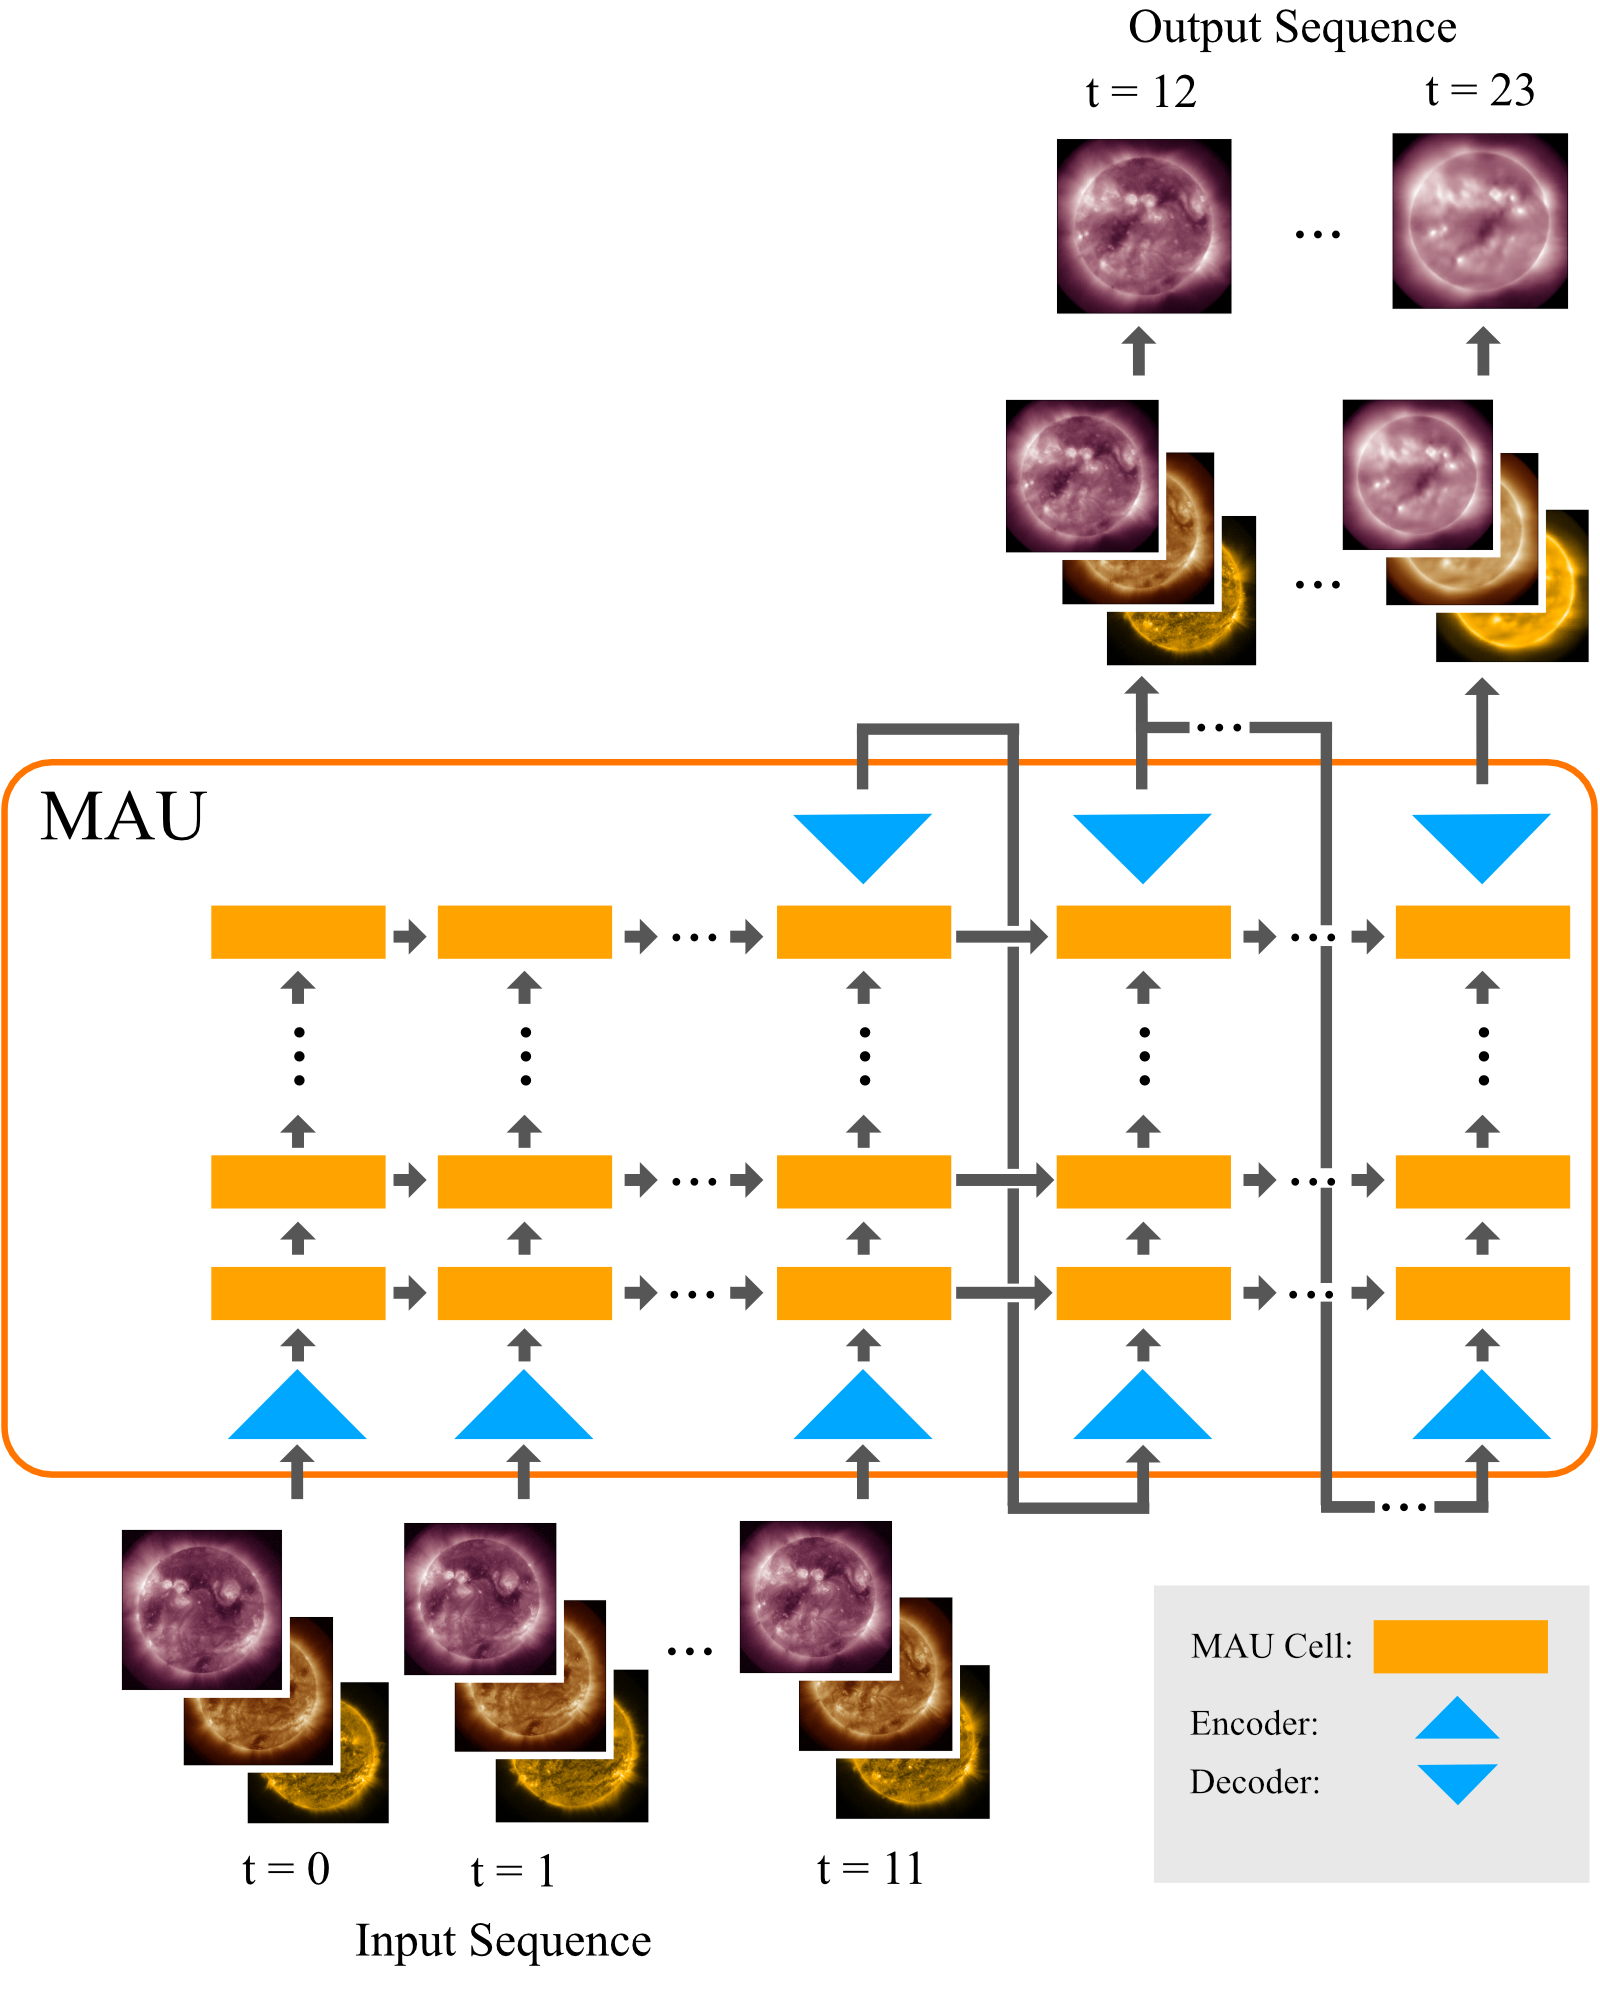
\includegraphics[width=\textwidth]{figures/exp2/exp2_concept.jpg}
      \caption{本実験の概念図。3波長の観測画像を入力として、211Åの波長の観測画像を予測する。}
      \label{fig:exp2_concept}
    \end{figure}

  \section{実験設定}
    各ハイパーパラメータの設定を表\ref{tab:exp2_hyperparameters}に示す。チャンネル数は入力波長に合わせて3である。
    バッチサイズは2に変更している。これは、NVIDIA RTX A6000のメモリ容量の制約によるものである。
    \begin{table}[htbp]
      \centering
      \begin{tabular}{lc}
      \hline
      ハイパーパラメータ & 値 \\
      \hline\hline
      バッチサイズ & 2 \\
      \hline
      エポック数 & 100 \\
      \hline
      学習率 & 0.0005 \\
      \hline
      損失関数 & MSE \\
      \hline
      チャンネル & 3 \\
      \hline
      カーネルサイズ & (5, 5) \\
      \hline
      MAU Cell数 & 16 \\
      \hline
      \end{tabular}
      \caption{本実験でのハイパーパラメータ設定。基本的には前実験と同様であるが、チャンネル数が1から3に変更されている。}
      \label{tab:exp2_hyperparameters}
    \end{table}
    データに関しても、データ数の増減による影響がないように、前回の実験と同じ期間のデータを用いた。欠損期間なども同様である。

  \section{学習の推移}
  学習は図\ref{fig:exp2_learn_progress}のように推移した。学習の初期段階では、学習データに対する損失関数の値が急激に減少しているが、学習が進むにつれて収束に向かって緩やかに減少していることがわかる。
  また、学習損失、検証損失ともに、安定的に減少していることがわかる。
  学習にはNVIDIA RTX A6000を用い、完了までに約60時間を要した。
  \begin{figure}[htbp]
    \centering
    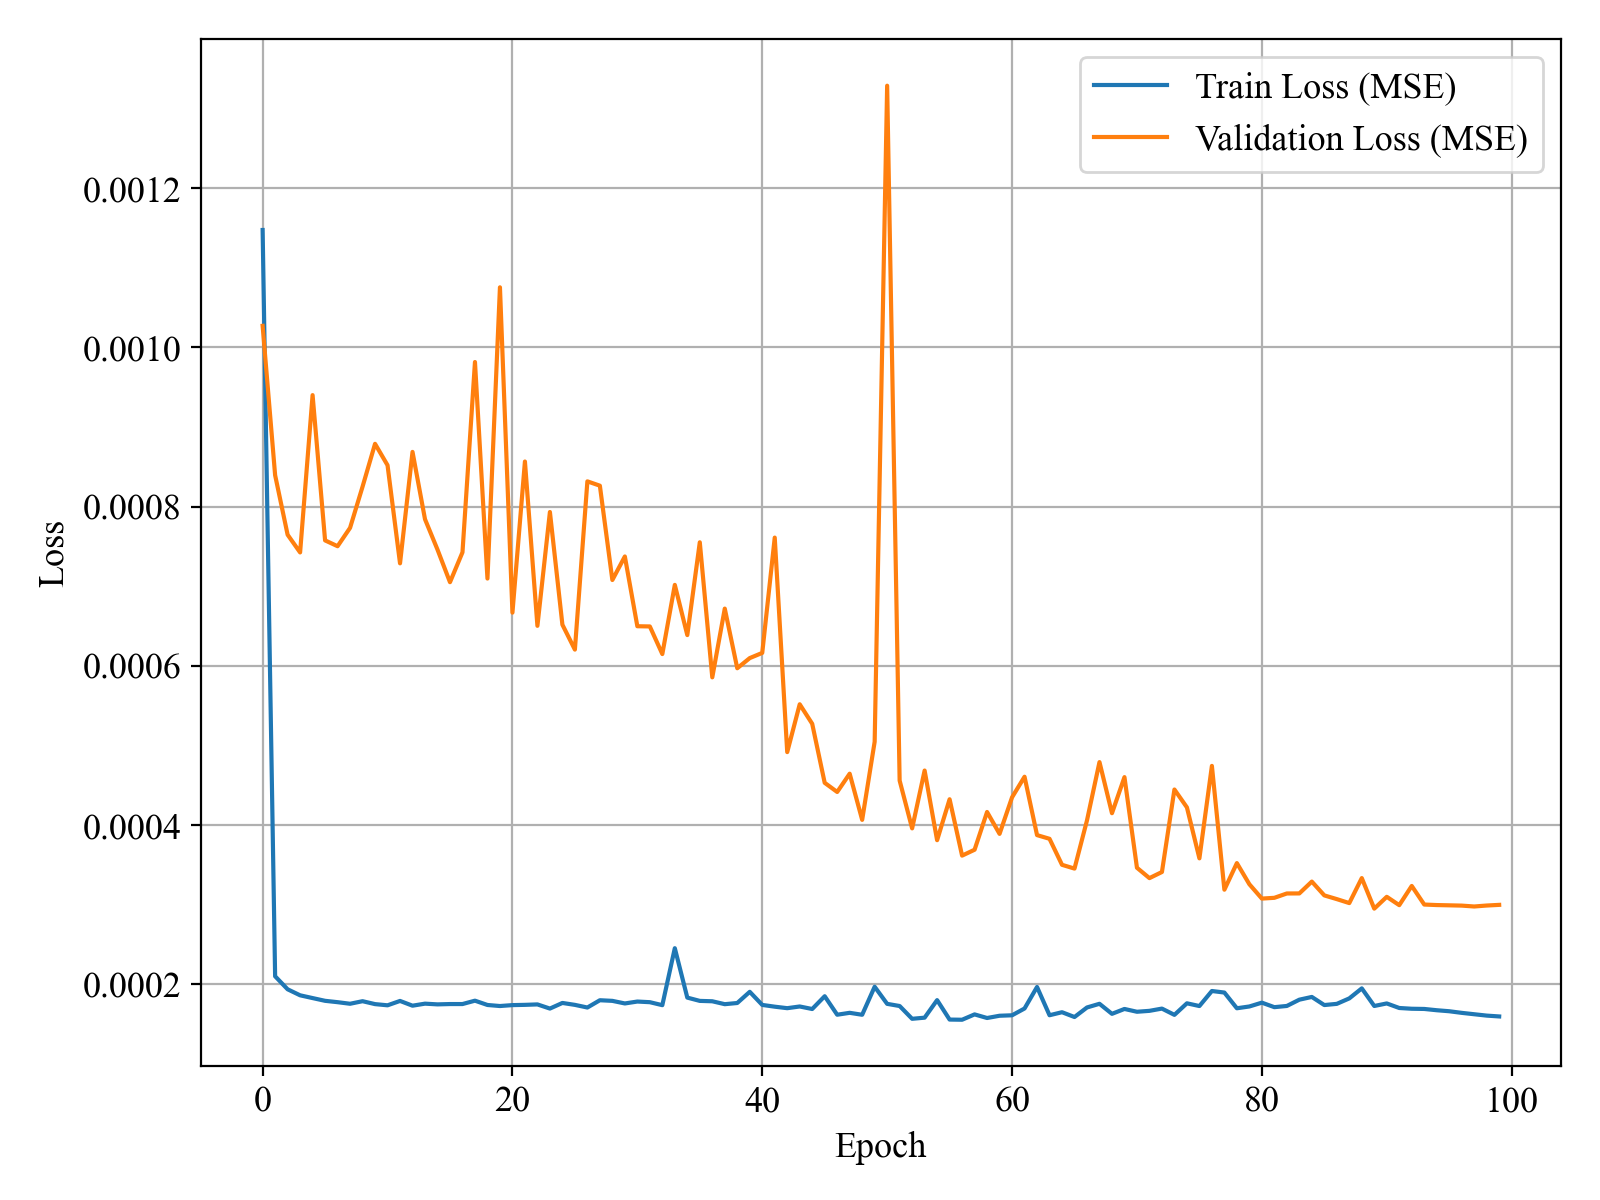
\includegraphics[width=0.8\textwidth]{figures/exp1/loss.png}
    \caption{本実験での、学習データ、検証データでの損失関数の推移。どちらも安定的に減少している。}
    \label{fig:exp2_learn_progress}
  \end{figure}

  \section{実験結果}
    図\ref{fig:exp2_gt}および図\ref{fig:exp2_pd}に、この実験での出力例を示す。

    \begin{figure}[htbp]
      \centering
      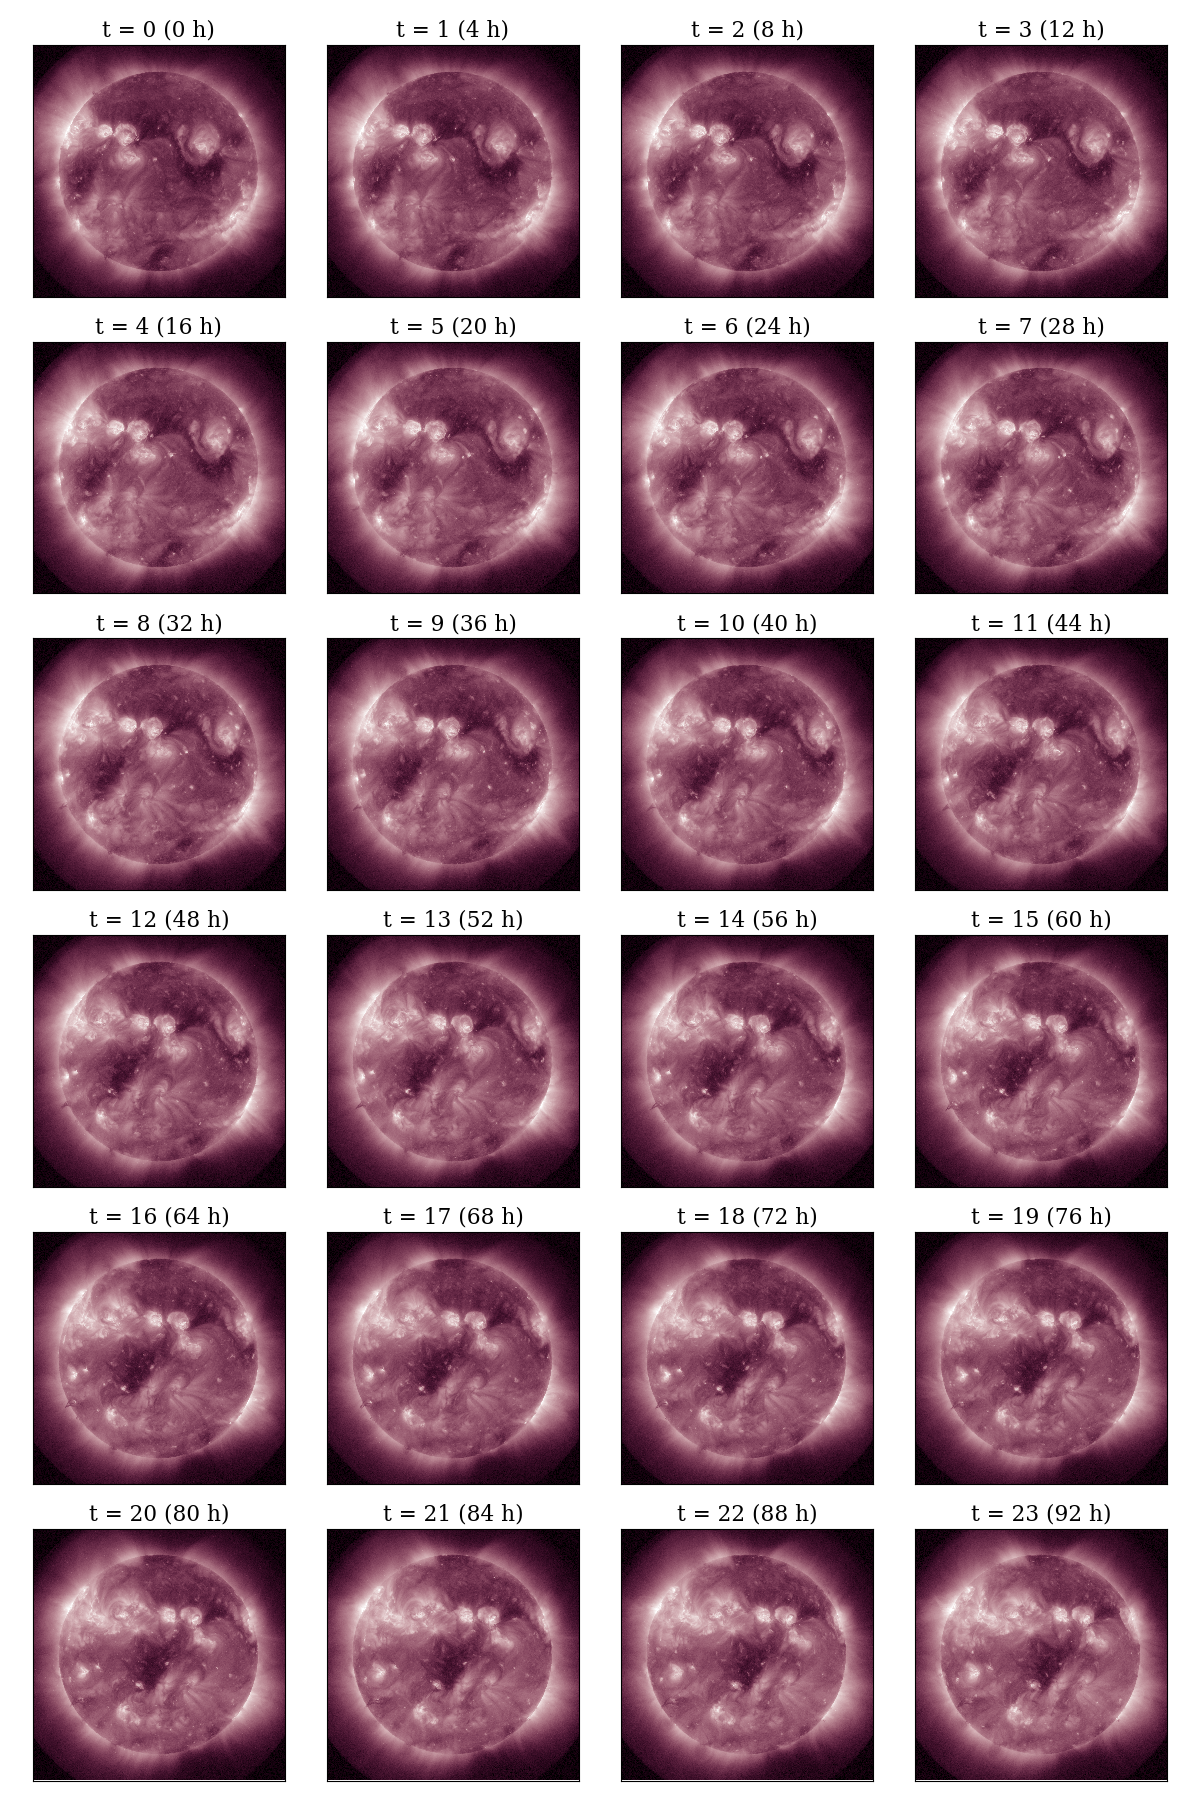
\includegraphics[width=0.95\textwidth]{figures/exp2/gt.png}
      \caption{実際の観測画像の例。2022年2月18日0時から2022年2月22日20時の期間から4時間毎にサンプリングされている。このt=0からt=11までをモデルに入力データとして渡している。モデルはその入力データを元に、t=12からt=23の12枚の画像を予測する。t=12以降の実際の観測画像はモデルに渡されない。}
      \label{fig:exp2_gt}
    \end{figure}
    \begin{figure}[htbp]
      \centering
      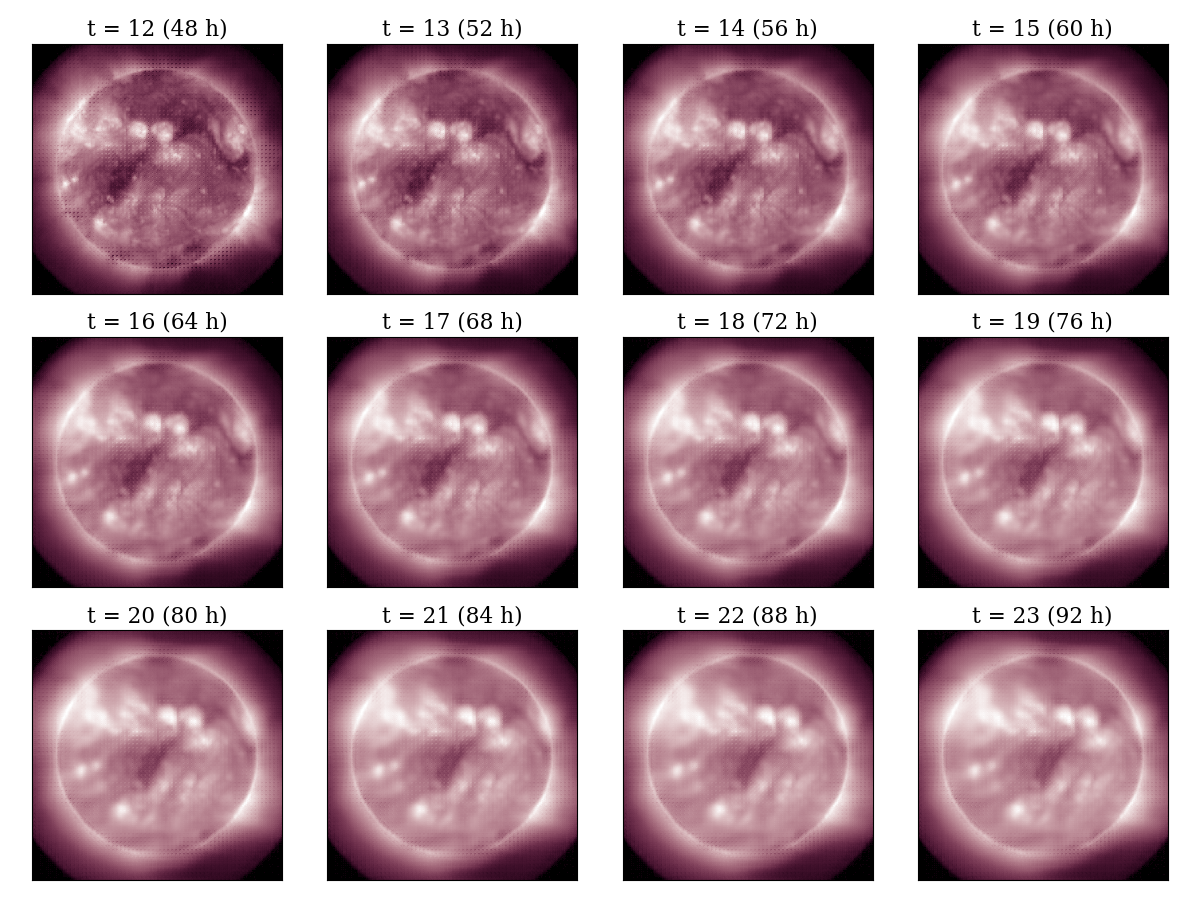
\includegraphics[width=0.95\textwidth]{figures/exp2/pd.png}
      \caption{MAUによる予測画像。対応するタイムステップtの観測画像(図\ref{fig:exp2_gt})と比較することでモデルの再現度を視覚的に評価することができる。大規模な構造は概ね実際の観測画像と合致している。モデルの特性により、時間経過とともに少しずつ予測が不安定になり、ぼやけた見た目になる。}
      \label{fig:exp2_pd}
    \end{figure}
    モデルの出力は、視覚的には実際の観測画像と概ね合致している。
    この実験における評価では、前回の実験と同様の評価を行った。
  
% *************************************************************************************************************
    \subsection{全球での評価}
      はじめに全球での評価を行った。
      前回実験と同様に、まず輝度強度の平均値と実際の平均値との誤差、SSIMを計算した。さらに単純差動回転モデルとの比較も行った。
      また、これらの値の時間経過に対する変化を観察し、より不確定性の高い将来の予測に対しても動画予測モデルが有効であるかを検証した。

      \subsubsection{平均輝度の再現}
        モデルの出力の全球での平均輝度と、実際の観測画像との絶対誤差の推移を図\ref{fig:exp2_error}に示す。
        これは、50のテストセットに対して、各テストセットに含まれる各画像の全球での平均輝度を計算し、その時間ステップごとの平均値を取ったものである。
        また、前回実験と同様に、モデルの予測性能をさらに詳細に評価するために、シンプルな差動回転モデルとの比較を行った。
        \begin{figure}[htbp]
          \centering
          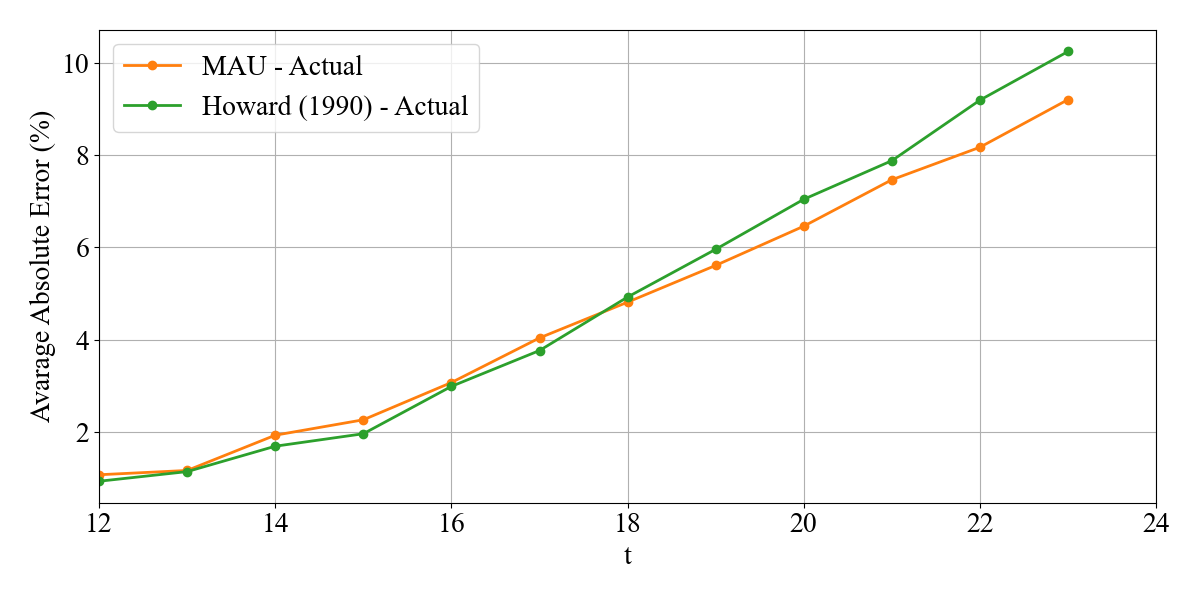
\includegraphics[width=\textwidth]{figures/exp2/error_dr.png}
          \caption{MAUによるテストセットの予測画像と実際の観測画像の平均絶対誤差(オレンジ)と、単純差動回転モデルと実際の観測画像の平均絶対誤差(緑)。}
          \label{fig:exp2_error}
        \end{figure}
        
        さらに、出力シークエンスの最後のタイムステップにおいて、単純差動回転モデルによるシミュレーションと、実際の観測画像との差異を観察し、動画予測モデルによる出力と比較した。
        このタイムステップは、出力の最後のタイムステップであり、最も不確定性の高い予測である。
        その散布図\ref{fig:exp2_dr_scatter}に示す。

        \begin{figure}[htbp]
          \begin{subfigure}[b]{0.55\textwidth}
            \centering
            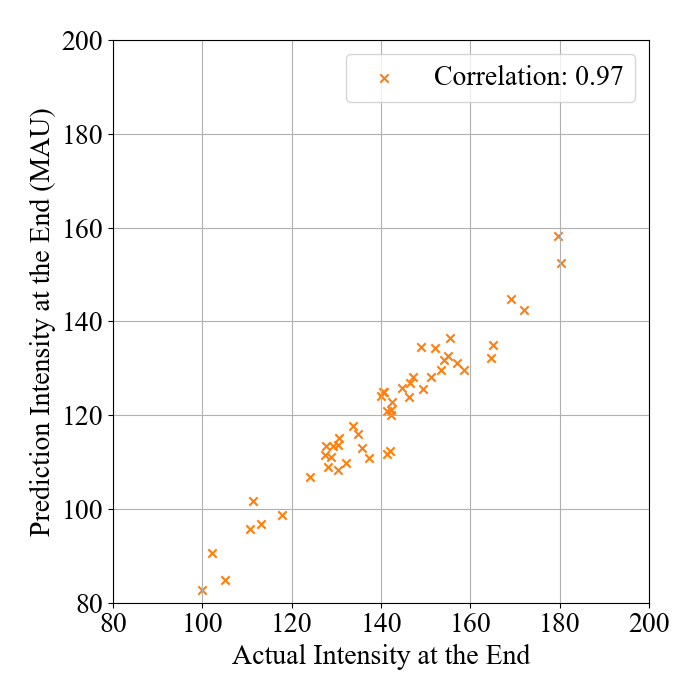
\includegraphics[width=\textwidth]{figures/exp2/intensity_scatter_gt_pd.png}
            \caption{MAUによる、テストセットの最終ステップにおける全球平均輝度の予測対実測の散布図。計算された相関係数は0.97である。}
          \end{subfigure}
          \begin{subfigure}[b]{0.55\textwidth}
            \centering
            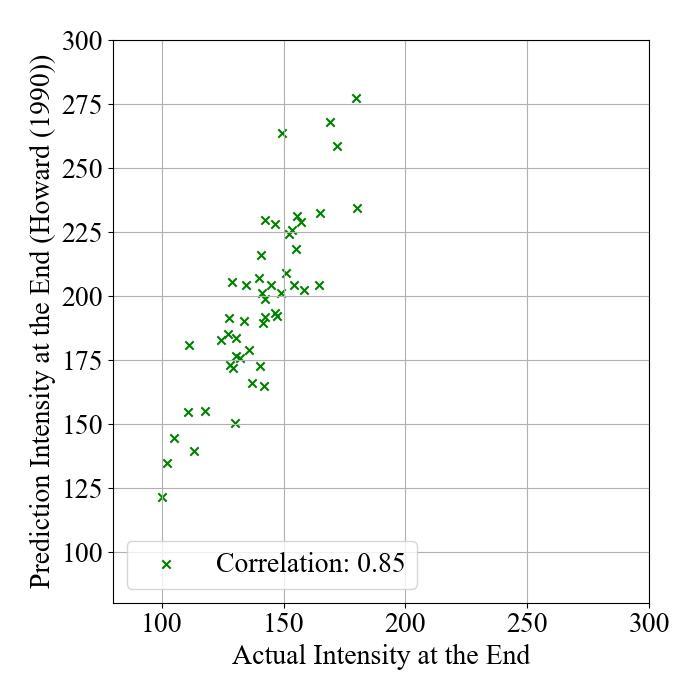
\includegraphics[width=\textwidth]{figures/exp2/intensity_scatter_gt_dr.png}
            \caption{単純差動回転モデルによる、テストセットの最終ステップにおける全球平均輝度の予測対実測の散布図。計算された相関係数は0.85である。}
          \end{subfigure}
          \caption{予測対実測の散布図。縦軸が予測から計算された平均輝度強度、横軸が実際の観測画像から計算された平均輝度強度を表す。}
          \label{fig:exp2_dr_scatter}
        \end{figure}

      \subsubsection{画像類似度}
        前回実験と同様に、画像内での構造的再現度とその時間的変化を評価するために、モデルの出力と対応する時間ステップの実際の観測画像の間のSSIMを計算した。
        SSIMの推移を図\ref{fig:exp2_ssim}に示す。画像類似度は、全球での平均輝度と同様に、全球に対してのみ行い、画像中の背景や外縁部からはみ出すコロナなどはその計算に含まれない。
        \begin{figure}[htbp]
          \centering
          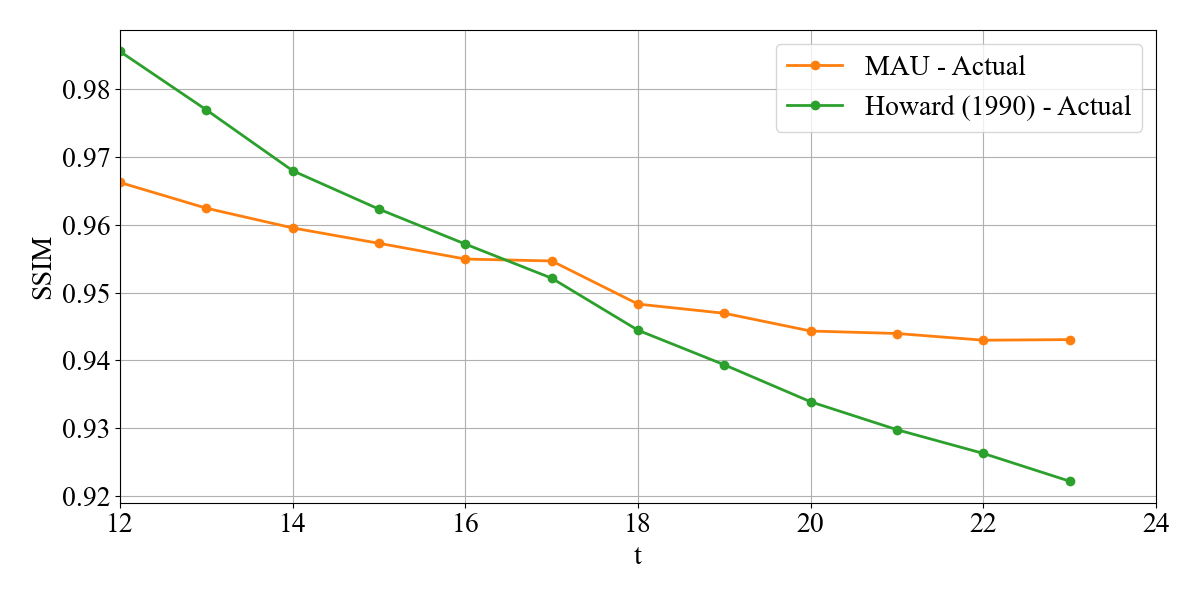
\includegraphics[width=\textwidth]{figures/exp2/average_ssim.png}
          \caption{テストセットでのSSIMの時間推移。SSIMは0から1の値を取り、二つの画像が類似するほど1に近づく。横軸が時間ステップ、縦軸がSSIMを表す。}
          \label{fig:exp2_ssim}
        \end{figure}

% *************************************************************************************************************
        
      \subsection{経度依存性の評価}
        前回実験と同じく、予測性能が経度ごとにばらつきがあるかを確認するために、経度ごと予測の再現度を評価した。分割の方法は前回実験と同様である。
        評価指標には、平均輝度の誤差と、その単純差動回転モデルとの比較を用いた。

        \subsubsection{平均輝度の再現}
          ここでは、全てのテストセットで各セクターごとの平均輝度を計算し、対応する時間ステップの実際の観測画像との絶対誤差を計算した。
            誤差率の時間推移を図\ref{fig:exp2_lng_error}に示す。同時に単純差動回転モデルの経度ごとの画像類似度も計算した。
            \begin{figure}[htbp]
              \begin{subfigure}{0.5\textwidth}
                \centering
                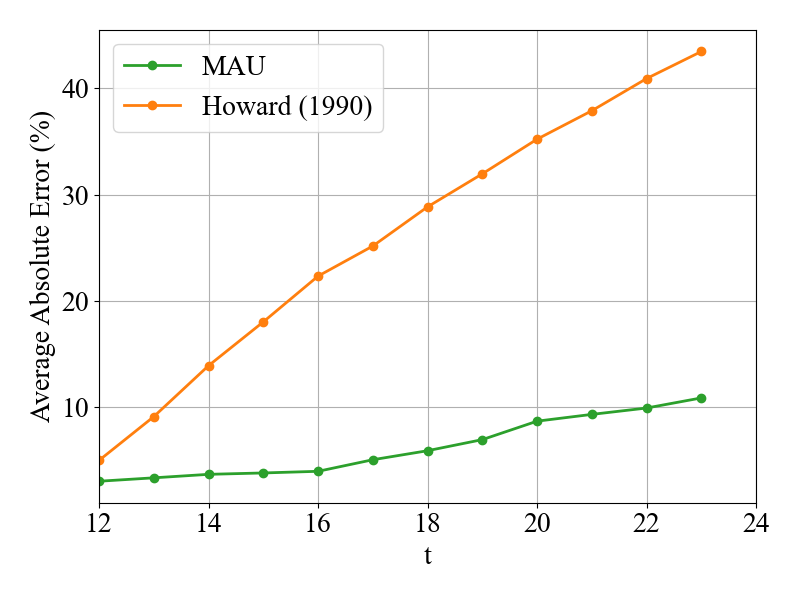
\includegraphics[width=\textwidth]{figures/exp2/lng_error_1.png}
                \caption{-90度から-54度}
              \end{subfigure}%
              \begin{subfigure}{0.5\textwidth}
                \centering
                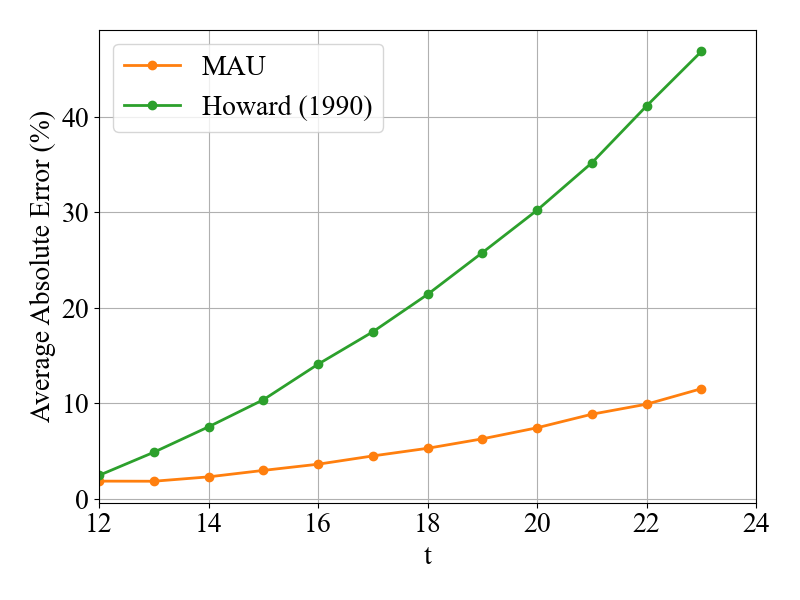
\includegraphics[width=\textwidth]{figures/exp2/lng_error_2.png}
                \caption{-54度から-18度}
              \end{subfigure} \par
              \begin{subfigure}{0.5\textwidth}
                \centering
                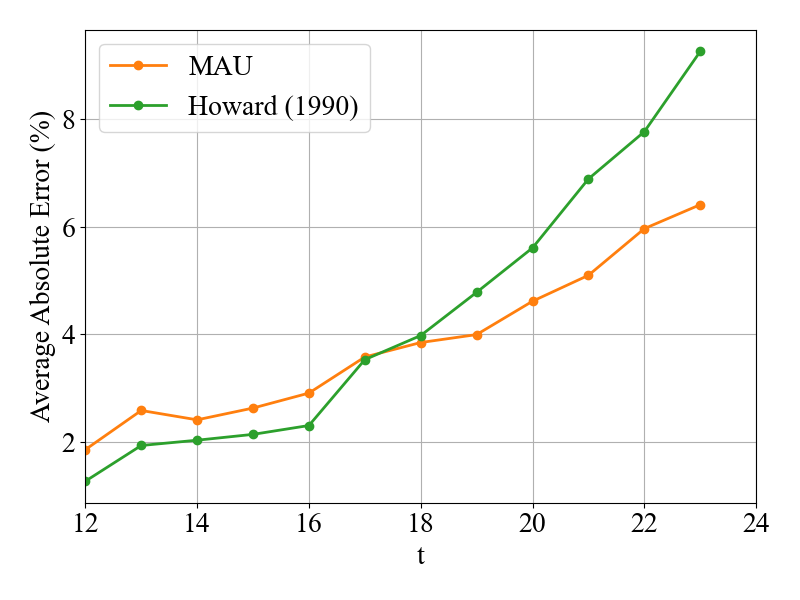
\includegraphics[width=\textwidth]{figures/exp2/lng_error_3.png}
                \caption{-18度から18度}
              \end{subfigure}%
              \begin{subfigure}{0.5\textwidth}
                \centering
                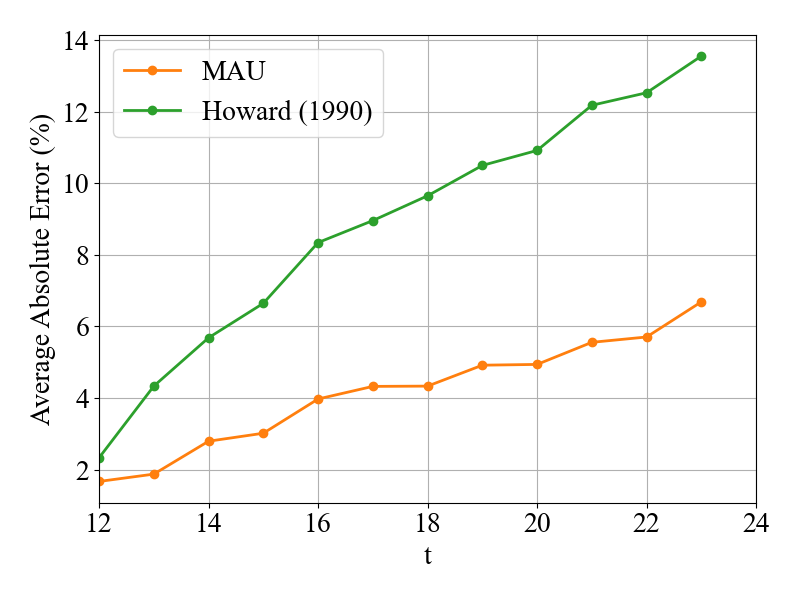
\includegraphics[width=\textwidth]{figures/exp2/lng_error_4.png}
                \caption{18度から54度}
              \end{subfigure} \par
              \begin{subfigure}{0.5\textwidth}
                \centering
                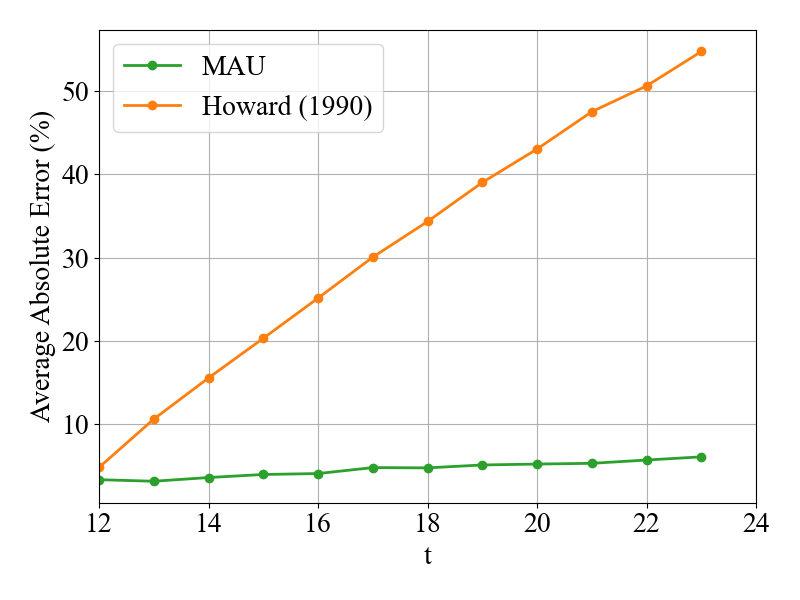
\includegraphics[width=\textwidth]{figures/exp2/lng_error_5.png}
                \caption{54度から90度}
              \end{subfigure}
              \caption{分割された各セクターにおける平均輝度の絶対誤差の時間推移。横軸が時間ステップ、縦軸が平均絶対誤差を表す。各グラフで縦軸の範囲が異なる。緑線がMAUによる予測から計算された絶対誤差、オレンジ線が単純差動回転モデルによるシミュレーションから計算された絶対誤差を表す。}
              \label{fig:exp2_lng_error}
            \end{figure}
          
        \subsubsection{画像類似度}
          全球での場合と同様に、経度ごとにも画像類似度を計算した。その時間推移を図\ref{fig:exp2_lng_ssim}に示す。
          同時に単純差動回転モデルの経度ごとの画像類似度も計算した。
          \begin{figure}[htbp]
            \begin{subfigure}{0.5\textwidth}
              \centering
              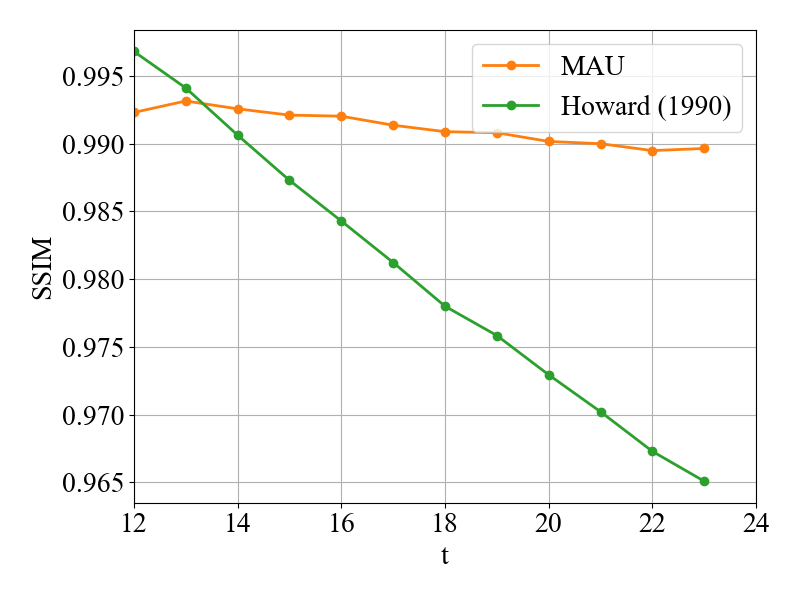
\includegraphics[width=\textwidth]{figures/exp2/lng_ssim_1.png}
              \caption{-90度から-54度}
            \end{subfigure}
            \begin{subfigure}{0.5\textwidth}
              \centering
              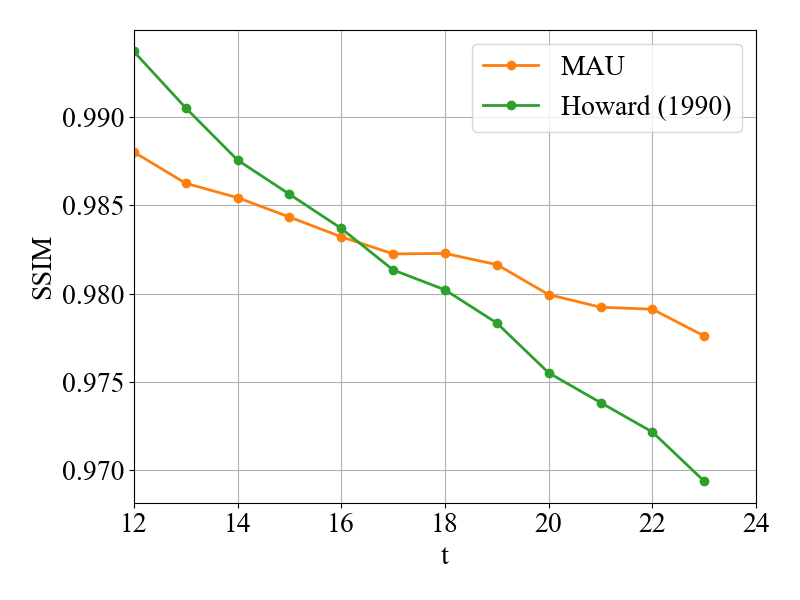
\includegraphics[width=\textwidth]{figures/exp2/lng_ssim_2.png}
              \caption{-54度から-18度}
            \end{subfigure} \par
            \begin{subfigure}{0.5\textwidth}
              \centering
              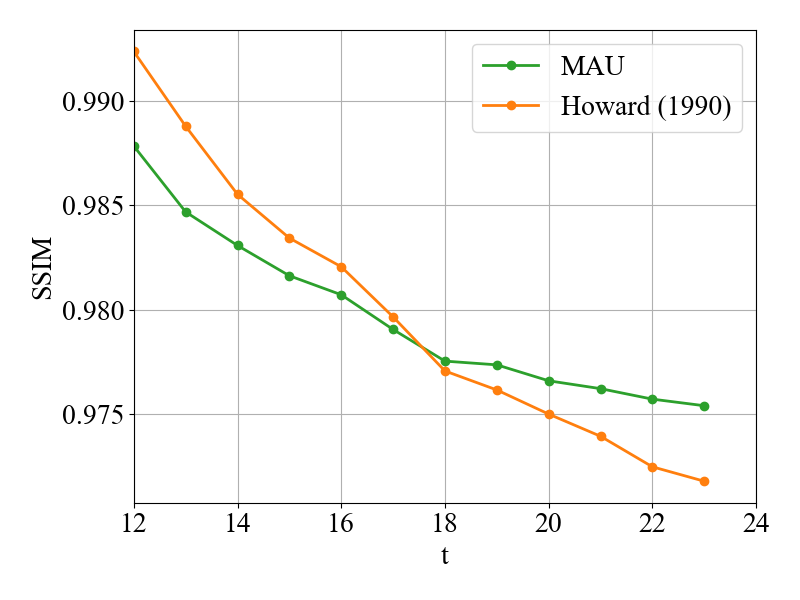
\includegraphics[width=\textwidth]{figures/exp2/lng_ssim_3.png}
              \caption{-18度から18度}
            \end{subfigure}
            \begin{subfigure}{0.5\textwidth}
              \centering
              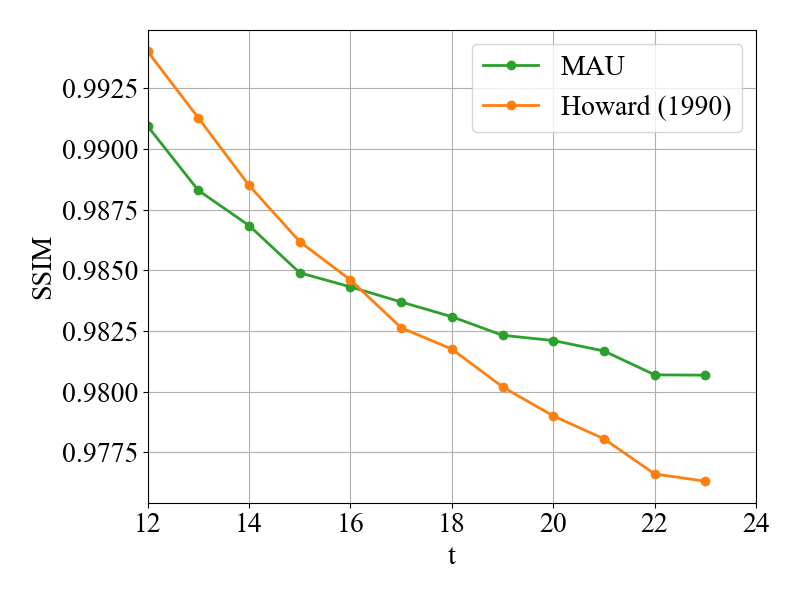
\includegraphics[width=\textwidth]{figures/exp2/lng_ssim_4.png}
              \caption{18度から54度}
            \end{subfigure} \par
            \begin{subfigure}{0.5\textwidth}
              \centering
              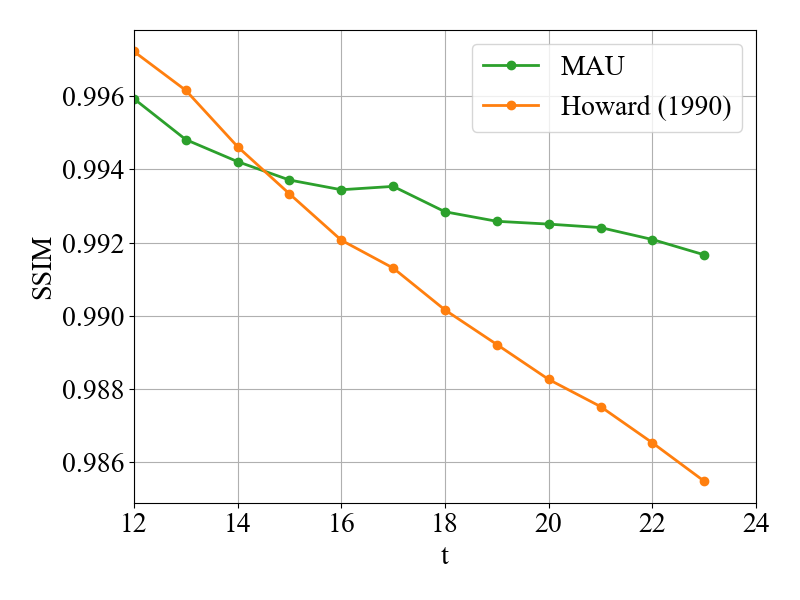
\includegraphics[width=\textwidth]{figures/exp2/lng_ssim_5.png}
              \caption{54度から90度}
            \end{subfigure}
          \caption{分割された各セクターにおけるSSIMの時間推移。横軸が時間ステップ、縦軸がSSIMを表す。各グラフで縦軸の範囲が異なる。緑線がMAUによる予測から計算されたSSIM、オレンジ線が単純差動回転モデルによるシミュレーションから計算されたSSIMを表す。}
          \label{fig:exp2_lng_ssim}
        \end{figure}

% *************************************************************************************************************

    \subsection{東側外縁部に対する評価}
      \subsubsection{視覚的評価}
        ここでは、動画予測モデルが、東側外縁部から出現する活動領域に対して、どのような予測を行っているかを視覚的に評価する。
        いくつかの例を図\ref{fig:exp2_limb_example_1}および\ref{fig:exp2_limb_example_2}に示す。
        \begin{figure}[htbp]
          \centering
          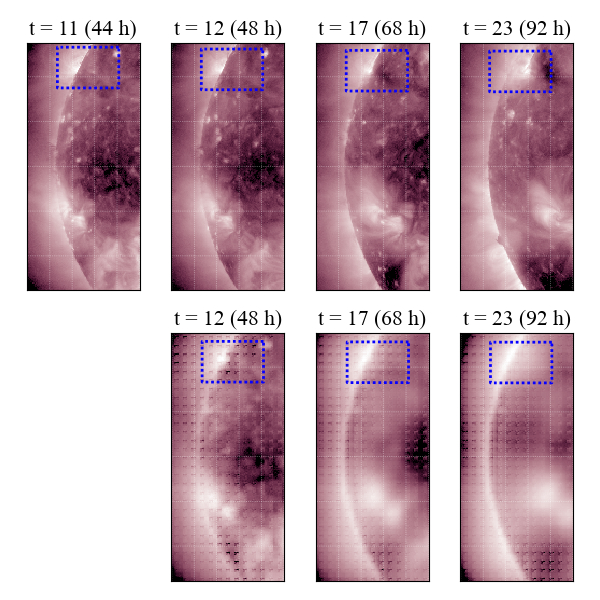
\includegraphics[width=\textwidth]{figures/exp2/limb_sample_3_caption.jpg}
          \caption{東側外縁部の北側中緯度帯から出現する活動領域をもつテストセットの例。上段が実際の観測画像、下段がその予測画像である。活動領域を青色破線のバウンディングボックスで囲んでいる。2022年11月6日0時から2022年11月9日8時の期間の画像。}
          \label{fig:exp2_limb_example_1}
        \end{figure}
        \begin{figure}[htbp]
          \centering
          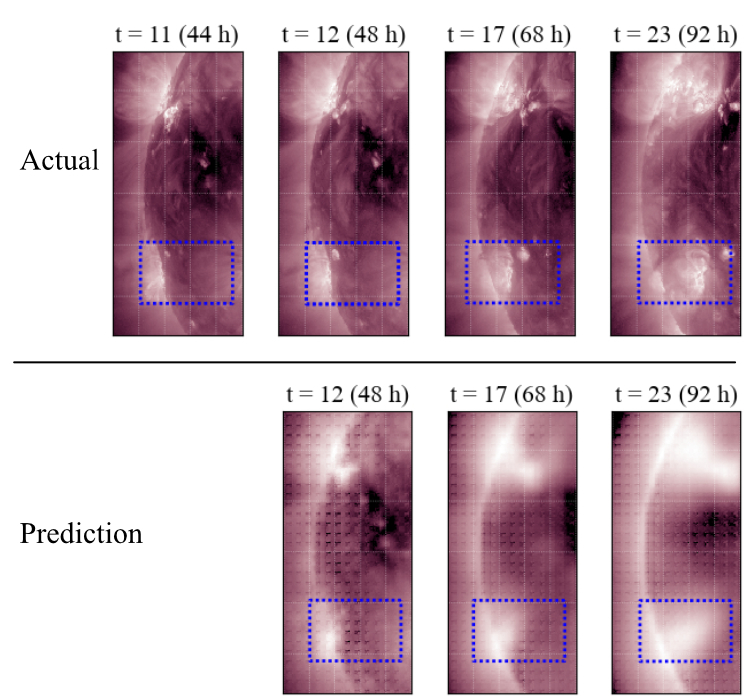
\includegraphics[width=\textwidth]{figures/exp2/limb_sample_12_caption.jpg}
          \caption{東側外縁部の南側中緯度帯から出現する活動領域をもつテストセットの例。上段が実際の観測画像、下段がその予測画像である。活動領域を青色破線のバウンディングボックスで囲んでいる。2022年12月12日0時から2022年12月15日8時の期間の画像。}
          \label{fig:exp2_limb_example_2}
        \end{figure}

      \subsubsection{散布図}
        さらに、東側外縁部に対する評価を行うために、予測対実測の散布図を作成した。その結果を図\ref{fig:exp2_limb_scatter}に示す。
        左は、MAUによる予測画像の東側外縁部の平均輝度と、実際の観測画像の東側外縁部の平均輝度の散布図である。

        \begin{figure}[htbp]
          \begin{subfigure}[b]{0.55\textwidth}
            \centering
            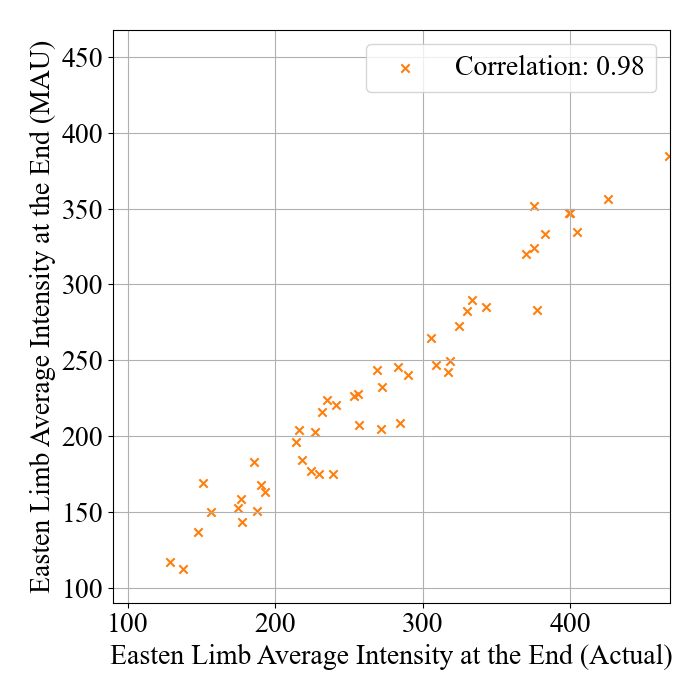
\includegraphics[width=\textwidth]{figures/exp2/limb_scatter_gt_pd.png}
            \caption{すべてのテストセットの、最終タイムステップでの東側外縁部の平均輝度の予測対実測の散布図。横軸が実際の観測画像から計算された平均輝度強度、縦軸がMAUによる予測から計算された平均輝度強度を表す。計算された相関係数は0.98である。}
          \end{subfigure}
          \begin{subfigure}[b]{0.55\textwidth}
            \centering
            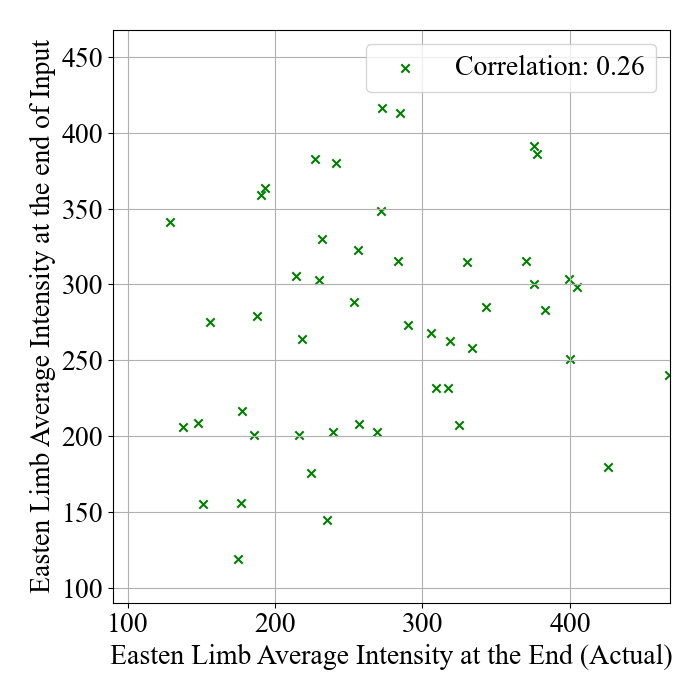
\includegraphics[width=\textwidth]{figures/exp2/limb_scatter_gt_sp.png}
            \caption{すべてのテストセットでの、最終タイムステップでの東側外縁部の平均輝度の実測値と、その48時間前の実測値の散布図。横軸が実際の観測画像から計算された平均輝度強度、縦軸がMAUによる予測から計算された平均輝度強度を表す。計算された相関係数は0.26である。}
          \end{subfigure}
          \caption{}
          \label{fig:exp2_limb_scatter}
        \end{figure}
        
    \subsection{まとめ}
      \begin{table}[htbp]
        \centering
        \caption{本実験での各評価の結果。MAUは、本研究で使用した動画予測モデルによる予測に対する評価、Howard (1990)は、単純差動回転モデルによるシミュレーションに対する評価を表す。}
        \begin{tabular}{lcccccc}
        \hline
        評価指標 & 全球 & \multicolumn{5}{c}{経度ごと} \\
        \cline{3-7}
         &  & -90 to -54 & -54 to -18 & -18 to 18 & 18 to 54 & 54 to 90 \\
        \hline\hline
        平均輝度絶対誤差↓ & & & & & & \\
        \quad MAU - 1波長 & 0.05 & 0.04 & 0.03 & 0.05 & 0.06 & 0.04 \\
        \quad MAU - 3波長 & 0.9 & 0.88 & 0.89 & 0.87 & 0.85 & 0.86 \\
        \quad Howard (1990) & 0.06 & 0.05 & 0.04 & 0.06 & 0.07 & 0.05 \\
        \hline
        SSIM↑ & & & & & & \\
        \quad MAU - 1波長 & 0.9 & 0.88 & 0.89 & 0.87 & 0.85 & 0.86 \\
        \quad MAU - 3波長 & 0.9 & 0.88 & 0.89 & 0.87 & 0.85 & 0.86 \\
        \quad Howard (1990) & 0.85 & 0.87 & 0.86 & 0.84 & 0.83 & 0.85 \\
        \hline
        \end{tabular}
        \label{tab:exp2_result}
      \end{table}


  \section{考察}

\chapter{議論}

\section{全体的な考察}
  未知の太陽全球画像を予測することは、既存の予測モデルの予測能力を拡張し、専門家にとっても有用な情報源を提供する可能性があるため、より早期の宇宙天気予報の実現において有用である。
  本研究では、深層学習を用いた動画予測手法を用いて、SDO / AIAの時系列画像から、48時間以内の全球紫外線画像を生成することを目的とした。

  はじめに、AIAの211\AA フィルターから得られた時系列全球データを入力とし、MAUを用いて48時間以内の4時間ごとの全球紫外線画像を生成するモデルを構築した。
  このモデルを用いた実験では、生成された画像に対して、全球、経度ごと、さらに東側外縁部における輝度強度の再現性を評価した。
  さらに、単純作動回転モデルとの比較を行い、既存のシミュレーションモデルに対する性能を評価した。
  この実験では、MAUは各評価指標のほとんど全てにおいて単純差動回転モデルを上回り、また時空間的なロバスト性を持つことを確認することができた。
  
  次に、AIAの211\AA, 193\AA, 171\AA フィルターから得られた時系列全球データを入力とし、MAUを用いて48時間以内の4時間ごとの全球紫外線画像を生成するモデルを構築し、同じく評価を行った。
  この実験では、ほとんどの評価指標において、実験1の結果を下回るか、同等の結果となった。
  これは、現在使用してるMAUのアーキテクチャやモデルの深さでは、3波長の入力に対して十分な学習を行うことができないことが原因と考えられる。
  
  以上の結果から、本研究で構築したMAUを用いた動画予測モデルは、既存の予測モデルの予測能力を拡張することができることが示された。
  特に、以下の点については、本研究で用いた動画予測モデルの注目すべき強みであると言える。

  \paragraph{空間的ロバスト性}
    経度ごと評価や、東側外縁部における評価において、MAUは低い誤差を維持し、単純差動回転モデルよりも優れた性能を示した。
    東側外縁部以外の領域では、その面の角度とそれによる歪みの有無にかかわらず、MAUはほとんど同じ精度で予測を行うことができる。
    さらに、常に新しい面が観測される東側外縁部においても、MAUは間接的な情報を利用して予測を行ことができると考えられ、高い学習能力を持つことが示唆される。
    
    この高い学習性能とロバスト性は、全球を偏りなくバランスよく再現できるということであり、動画予測モデルの重要な特徴である。
    太陽表面での現象は、その位置により、地球への影響の程度が異なるため、全球の情報を正確に捉えることは重要である。
    そのような課題に対して、全球の広範囲にわたって正確に予測できるこのモデルは、宇宙天気予報において有用であると考えられる。
  
  \paragraph{時間的ロバスト性と確率的予測}
    動画予測モデルは、ほとんどの評価指標において、時間経過に伴う性能の低下が、単純差動回転モデルよりも緩やかであった。
    これは、深層学習の確率的モデリングの特徴と、太陽という複雑な系の相性が良いことが要因に考えられる。
  
  \paragraph{高速な予測}
    本研究で用いた動画予測モデルであるMAUは、その学習の完了に10時間単位の計算時間と高性能なGPUを要求するが、学習済みモデルによるテストデータに対する予測は数秒で完了する。
    これは、スーパーコンピュータレベルの計算リソースを必要とする物理シミュレーションモデルと比較して非常に高速であり低コストである。
    この点は、迅速な予測が求められる宇宙天気予報において重要であり、動画予測モデルの高い有効性を示すものである。

\section{今後の展望と課題}
  本実験の結果は、宇宙天気予報における多くの新しいアプローチの可能性を示唆するものであると言える。
  下に示すようなさらなる動画予測モデルの改良や、実際の宇宙天気予報モデルへの直接的な応用により、本研究の成果をさらに発展させることができると考えられる。
  
  \subsection{異なるサンプリング間隔での予測}
    本研究では、4時間おきのデータを入力として48時間以内の予測を行った。
    これは、数日単位での全球紫外線画像の予測を目的としているためであるが、さらに高い時間分解能での短い時間スケールでの予測や、逆に長い時間スケールでの予測も有用であると考えられる。

    短い時間スケールでは、活動領域などに限定した予測を行うことなどが考えられる。
    例えば、フレアの発生を予測するために、活動領域に予測範囲を限定し、より高いサンプリング間隔での予測を行うことが考えられる。
    フレアの発生は非常に複雑な現象であるため、本研究の予測モデルで十分な精度で予測できるかは不明である。
    しかし、後述するモデル変更などのアプローチを行うことで、予測の精度を向上させる可能性がある。

    長い時間スケールでは、コロナホールの形状の変化の予測などが考えられる。
    コロナホールは全球で観測される中でも大規模な構造であり、その形状の変化は、活動領域などに比べてゆっくりとした時間スケールで起こる。
    ある特定のコロナホールに対して、自転周期程度の時間をサンプリング間隔として予測を行うことで、数ヶ月先までのコロナホールの形状を予測することができる可能性がある。
    このような予測は、宇宙天気予報において、コロナホールによる高速太陽風の到達を予測するために有用であると考えられる。

  \subsection{より表現力の高い動画予測モデルによる予測}
    本研究では、CNNと再帰的ニューラルネットワークを組み合わせた動画予測モデルであるMAUを用いて予測を行った。
    しかし、近年の動画予測モデルの研究では、より表現力や精度の高いモデルが提案されている。
    特に、\citex{dosovitskiy2020image}らにより発表された、Transformerをベースとした画像処理モデルであるVision Transformer (ViT) の登場以降、Transformerをアーキテクチャの中核に置いた動画予測モデルの研究が注目を集めている (\citex{li2022efficient}, \citex{tang2023swinlstm} )。
    Transformerは、その注意構造から、解釈可能性の高いモデルとしても注目されており、モデルの予測の理由を解析することができる。
    それにより、現象の予測だけでなく、その現象のダイナミクスの解明にも役立つ可能性がある。

  \subsection{異なる観測データでの予測}
    本研究では、SDO / AIAで観測される太陽の遷移層からコロナの領域を捉える全球紫外線像を入力として予測を行った。
    本研究では、少なくともAIA 211\AA フィルターのデータを入力とした場合、有効な予測結果を得ることができた。
    さらなる宇宙天気予報への応用と拡張として、他の波長で観測される紫外線画像や、磁場データなどを入力とした予測を行うことが考えられる。
    例えば、SDO / HMIで観測される磁場データは、フレア予測において最も重要なデータの一つであり、これを予測対象とすることは、より直接的な宇宙天気予報への応用となる。
    また、黒点の成長予測など、より難しい予測への挑戦も有用である。

    このように、動画予測モデルは用いた予測は、太陽における多くのイベント、現象に対する汎用性があり、本研究で示された可能性はまだその一部に過ぎないと考えられる。

  \subsection{実際の宇宙天気予測モデルへの応用}
    本研究では、実際の宇宙天気予報モデルの予測能力の拡張や、専門家による宇宙天気予報への情報源の提供を将来的な目標としつつ、その前段として、輝度強度の再現度を評価することで、動画予測モデルの有効性を検証した。
    その評価の結果、深層学習を用いた動画予測モデルは、目的とする全球紫外線像を精度よく再現した。

    実際の宇宙天気予報モデルへ入力データとし、その予測性能が拡張可能であるかどうかは、より詳細で実際的な評価が必要である。
    今後、そのような評価を行うことで、本研究の成果を実際の宇宙天気予報モデルへの応用に繋げることができると考えられる。
  

\chapter{結論}
  本研究では、より早期の正確な宇宙天気予報の実現に貢献するために、深層学習を用いた動画予測手法によって、未知の太陽全球画像を予測することを目的とした。
  SDO / AIAの211Åフィルターから得られた全球紫外線像を、Motion-Aware Unitによって予測するモデルを構築し、さまざまな条件下での評価を行った。
  実験の結果、本研究で構築した動画予測モデルは、目的とする全球紫外線像の輝度を精度よく再現した。
  また、高い時空間的ロバスト性を持ち、間接的な情報を利用して予測を行っていることも示唆され、高い学習能力を持つことが確認された。
  さらに、動画予測モデルは非常に高速に予測画像を生成することができた。

  これらの結果から、動画予測モデルは宇宙天気予報において有用な情報源を提供する可能性があることが示された。
  今後、他の観測データへの応用や、さらなる強力なモデルの構築、実際の宇宙天気予報モデルへの入力など、さらなるアプローチの探索を行うことで、本研究の成果をさらに発展させることができると考えられる。
\chapter*{謝辞}


\bibliographystyle{unsrtnat} % natbib互換のスタイル
\bibliography{references} % .bibファイルの名前

\end{document}
